\section[\texorpdfstring{$\textup{N}^3\textup{LO}$ QCD corrections and resummation}{N3LO QCD corrections and resummation}]{\texorpdfstring{\boldmath$\textup{N}^3\textup{LO}$ QCD corrections and resummation}{N3LO QCD corrections and resummation}}
\label{sec:n3lo-qcd}

This section combines results from several publications. In the HTL, the N$^3$LO QCD corrections to the inclusive total cross section and the Higgs boson pair invariant-mass ($m_{hh}$) distribution were first reported in Refs.~\cite{Chen:2019lzz, Chen:2019fhs}. The N$^3$LL soft-gluon threshold resummation for the same observables was presented in Ref.~\cite{Ajjath:2022kpv}. More recently, fully differential N$^3$LO QCD calculations were presented in Ref.~\cite{Chen:2026zmi}.

In the HTL, the effective Lagrangian for the
coupling of the Higgs field to two gluon field strength tensors
can be written as
\begin{align}\label{eq:effL}
 \mathcal{L}_{\rm eff}= -\frac{1}{4}  G_{\mu\nu}^a G^{a~\mu\nu}
 \left(
  C_{h} \frac{h}{v} - C_{hh} \frac{h^2}{2v^2}
 \right)\,,
\end{align}
where $v$ is the Higgs vacuum expectation value and
$C_h$, $C_{hh}$ are the Wilson coefficients obtained by matching the full Standard Model (SM) onto the effective theory, in which the top quark degree of freedom has been integrated out.
The Wilson coefficients start at $\mathcal{O}(\alpha_s)$ and are known up to $\mathcal{O}(\alpha_s^4)$~\cite{Inami:1982xt, Chetyrkin:1997iv, Chetyrkin:1997un, Schroder:2005hy, Chetyrkin:2005ia, Kniehl:2006bg,Baikov:2016tgj,Spira:2016zna,Gerlach:2018hen}.

In this section, we present our theoretical predictions using the following setup~\cite{Chen:2019lzz,Chen:2019fhs,Ajjath:2022kpv,Chen:2026zmi}. We take the Higgs-boson mass $m_h=125$ GeV, the top quark pole mass $m_t=173$ GeV, and the Higgs vacuum expectation value $v=246.2$ GeV. We employ either the \texttt{PDF4LHC15\ttus nnlo\ttus 30}~\cite{Butterworth:2015oua,Dulat:2015mca,Harland-Lang:2014zoa,NNPDF:2014otw} or the \texttt{PDF4LHC21\ttus 40}~\cite{PDF4LHCWorkingGroup:2022cjn}
(\texttt{NNPDF40\ttus an3lo\ttus as\ttus 01180}~\cite{NNPDF:2024nan}) parton distribution function (PDF) sets for observables without and with fiducial cuts, respectively, together with the corresponding $\alpha_s$ running provided by {\tt LHAPDF6}~\cite{Buckley:2014ana}.\footnote{We note here that the N$^3$LO $k$-factors in the final recommendations of Section~\ref{sec:recs} were produced using the \texttt{PDF4LHC21\ttus 40} set.}
The central renormalization and factorization scales are chosen as $\mu_0 = m_{hh}/2$. Scale uncertainties, which estimate missing higher-order corrections, are obtained from the envelope of the $7$-point variations of
$\mu_F$ and $\mu_R$, defined as $\mu_{R/F} = \xi_{R/F} \mu_0$ with $\xi_{R/F}\in \left\{0.5,1,2\right\}$, excluding the two extreme combinations $(\xi_R, \xi_F)=(0.5, 2)$ and $(2, 0.5)$. We quote only the scale uncertainty, since other parametric uncertainties are largely independent of the perturbative order.
For the fully differential results, we impose the following fiducial cuts~\cite{Chen:2026zmi}:
\begin{equation}
\label{eq:fiducialcuts}
p_{T, h_{1}}>30~\mathrm{GeV}\,, \quad p_{T, h_{2}}>20~\mathrm{GeV}\,, \quad |y_{h}|<2.4\,,
\end{equation}
where $h_1$ and $h_2$ denote the leading and subleading Higgs bosons, ordered by their transverse momenta $p_{T,h_i}$.

\subsection[\texorpdfstring{$\textup{N}^3\textup{LO}$ in the HTL}{N3LO in the HTL}]{\texorpdfstring{\boldmath$\textup{N}^3\textup{LO}$ in the HTL}{N3LO in the HTL}}

%\textit{Authors:} Long-Bin Chen, Hai Tao Li, Hua-Sheng Shao, Jian Wang (1909.06808)

\textbf{Long-Bin Chen, Xuan Chen, Yuesheng Dai, Hai Tao Li, Shi-Yuan Li, Hua-Sheng Shao, Jian Wang~\cite{Chen:2019lzz,Chen:2026zmi}.}



\begin{figure}[!hbtp]
    \centering
    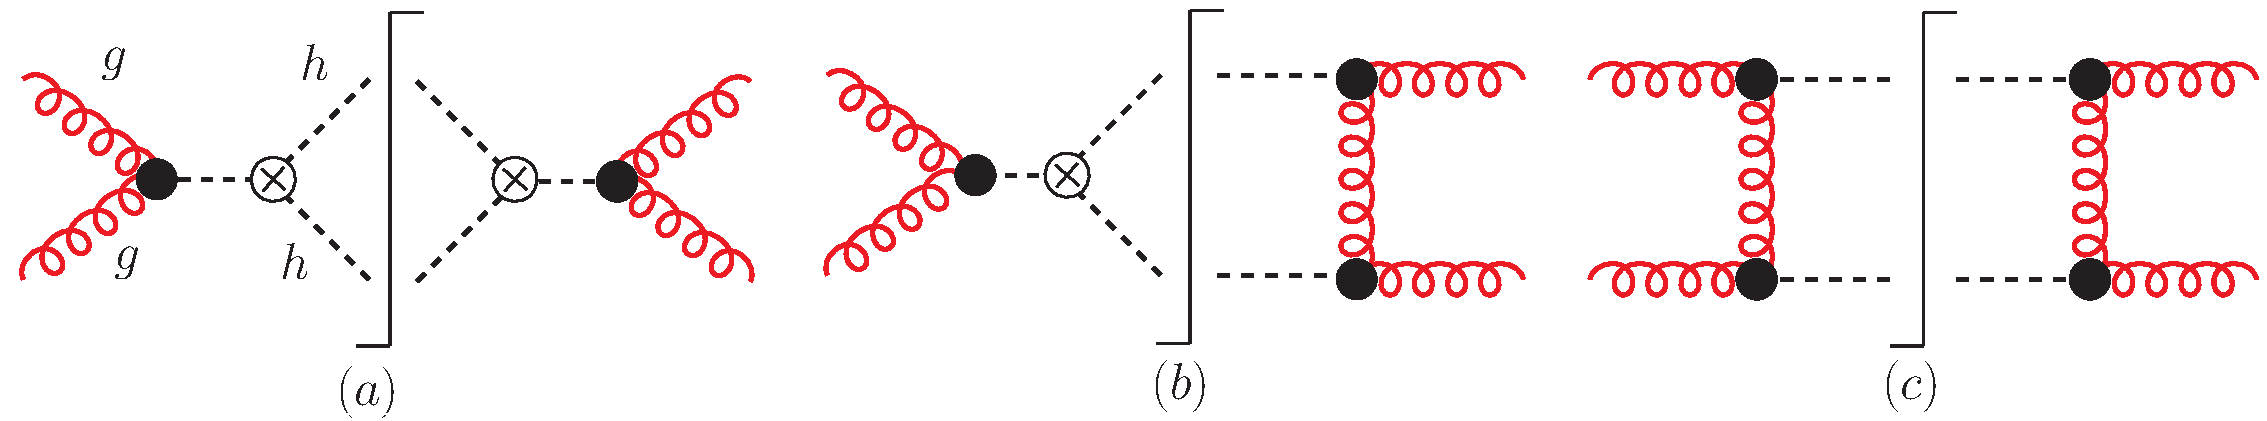
\includegraphics[width=\textwidth]{N3LO_QCD_SM/N3LO_htl/Images/feyn_HH}
    \caption{Representative Born-level cut diagrams for Higgs boson pair production via gluon-gluon fusion. Bullets denote the effective vertices described by the Lagrangian in Eq.~\eqref{eq:effL}, while the crossed circle represents the trilinear Higgs boson self-coupling. Figure adapted from Ref.~\cite{Chen:2019lzz}.}
    \label{fig:FeynDia}
\end{figure}

\noindent The fixed-order computation of the gluon-gluon fusion (ggF) Higgs boson pair cross section in the HTL can be organized according to the number of the effective-vertex insertions in the squared amplitude. Three representative Born-level cut diagrams are shown in Fig.~\ref{fig:FeynDia}: from left to right, they involve two, three, and four effective vertices, and are denoted as class-$a$, class-$b$, and class-$c$ contributions, respectively. Accordingly, the phase-space-integrated or differential cross section can be decomposed as
\begin{align}
    d\sigma_{hh} = d\sigma^{a}_{hh} + d\sigma^{b}_{hh} + d\sigma^{c}_{hh} .
\end{align}
Their contributions at different powers of $\alpha_s$ are summarized in Table~\ref{tab:my_label}. To achieve N$^3$LO accuracy in $\alpha_s$, the required inputs are the class-$a$ contribution at $\mathrm{N^3LO}_a$, the class-$b$ contribution at $\mathrm{NNLO}_b$, and the class-$c$ contribution at $\mathrm{NLO}_c$, where the subscripts indicate the perturbative order within the corresponding topology class.

\begin{table}[hbt!]
    \centering
%    \begin{tabular}{c|c|c|c|c}
%    \begin{tabular}{ccccc}
%%    \hline \hline
%    \toprule
%        &  LO  & NLO  & NNLO  & $\textup{N}^3\textup{LO}$  \\
%%    \hline
%    \midrule
%    Class  &  $\mathcal{O}(\alpha_s^2)$  &   $\mathcal{O}(\alpha_s^3)$ &   $\mathcal{O}(\alpha_s^4)$  & $\mathcal{O}(\alpha_s^5)$
%     \\
%%    \hline
%    \midrule
%    \multirow{2}{*}{$a$}
%     &  $\textup{LO}_a$  &   $\textup{NLO}_a$ &   $\textup{NNLO}_a$  & $\textup{N}^3\textup{LO}_a$
%     \\
%      &  $\mathcal{O}(\alpha_s^2)$  &   $\mathcal{O}(\alpha_s^3)$ &   $\mathcal{O}(\alpha_s^4)$  & $\mathcal{O}(\alpha_s^5)$
%     \\
%%    \hline
%    \midrule
%     \multirow{2}{*}{$b$}
%     &  --- &   $\textup{LO}_b$ &   $\textup{NLO}_b$  &  $\textup{NNLO}_b$
%     \\
%     &  0 &   $\mathcal{O}(\alpha_s^3)$ &   $\mathcal{O}(\alpha_s^4)$  & $\mathcal{O}(\alpha_s^5)$
%     \\
%%    \hline
%    \midrule
%    \multirow{2}{*}{$c$}
%      & --- &  --- &   $\textup{LO}_c$  & $\textup{NLO}_c$
%     \\
%       & 0 &  0 &   $\mathcal{O}(\alpha_s^4)$  & $\mathcal{O}(\alpha_s^5)$
%     \\
%%     \hline \hline
%    \bottomrule
%    \end{tabular}
\begin{tabular}{ccccc}
    \toprule
        \multirow{2}{*}{Class}    &  LO  & NLO  & NNLO  & $\textup{N}^3\textup{LO}$  \\
      &  $\mathcal{O}(\alpha_s^2)$  &   $\mathcal{O}(\alpha_s^3)$ &   $\mathcal{O}(\alpha_s^4)$  & $\mathcal{O}(\alpha_s^5)$
     \\
    \midrule
    $a$ &  $\textup{LO}_a$  &   $\textup{NLO}_a$ &   $\textup{NNLO}_a$  & $\textup{N}^3\textup{LO}_a$
     \\
     $b$ &  --- &   $\textup{LO}_b$ &   $\textup{NLO}_b$  &  $\textup{NNLO}_b$
     \\
    $c$ & --- &  --- &   $\textup{LO}_c$  & $\textup{NLO}_c$
     \\
    \bottomrule
    \end{tabular}
            \caption{Perturbative orders in $\alpha_s$ for three topology classes.
    The first and second rows indicate the perturbative expansion orders of the total cross section for Higgs boson pair production,
    while each individual class has its own expansion order, specified by the subscript.}
    \label{tab:my_label}
\end{table}

The class-$a$ contribution can be obtained from the single-Higgs production cross section in the HTL up to N$^3$LO.
For inclusive results, this component is computed using the public program \texttt{iHixs2}~\cite{Dulat:2018rbf}, while the class-$a$ contribution for fully differential results is computed with \texttt{NNLOJet}~\cite{NNLOJET:2025rno} using the $q_T$ phase-space slicing ($q_T$-slicing) method~\cite{Catani:2007vq,Cieri:2018oms}.
The class-$b$ contribution is calculated up to NNLO in $\alpha_s$ using the $q_T$-slicing method~\cite{Catani:2007vq} by combining the \texttt{MadGraph5\_aMC@NLO}~\cite{Alwall:2014hca,Frederix:2018nkq} framework with a private code. The corresponding two-loop amplitude with two effective-vertex insertions was computed in Ref.~\cite{Banerjee:2018lfq}. The double-real and real-virtual contributions in class-$b$, as well as all contributions in class-$c$, are calculated using \texttt{MadGraph5\_aMC@NLO}.

\begin{table}[h]
\begin{center}

\newcolumntype{P}[1]{>{\centering\arraybackslash}p{#1}}
{\renewcommand{\arraystretch}{1.5}
%\begin{tabular}{|P{2.7cm}|P{2.7cm}|P{2.7cm}|P{2.7cm}|}
\begin{tabular}{P{2.7cm}P{2.7cm}P{2.7cm}P{2.7cm}}
\toprule
    & $\sigma_{{\rm NLO}}$ $[\textup{fb}]$
    & $\sigma_{{\rm NNLO}}$ $[\textup{fb}]$
    & $\sigma_{{\rm N}^3{\rm LO}}$ $[\textup{fb}]$
    \\
  \midrule
  Inclusive &
  $31.89^{+18\%}_{-15\%}$ &
  $37.55^{+5.2\%}_{-7.6\%}$ &
 $38.65^{+0.5\%}_{-2.7\%}$
 \\
 \midrule
   Fiducial &
  $27.87_{-15 \%}^{+18 \%}$ &
  $32.74_{-7.3 \%}^{+5.2 \%}$ &
 $34.00(4)_{-2.9 \%}^{+1.4 \%}$
 \\
 \bottomrule
\end{tabular}}
\caption{Fixed-order cross sections in the HTL at $\sqrt{s}=14\,\textup{TeV}$. The second line corresponds to the inclusive case, while the third line corresponds to the fiducial case with cuts defined in Eq.~\eqref{eq:fiducialcuts}. The quoted uncertainties are obtained from $7$-point scale variations.}
\label{tab:FON3LOinclusivexs}
%\end{small}
\end{center}
\end{table}

\begin{figure*}[t]
\centering
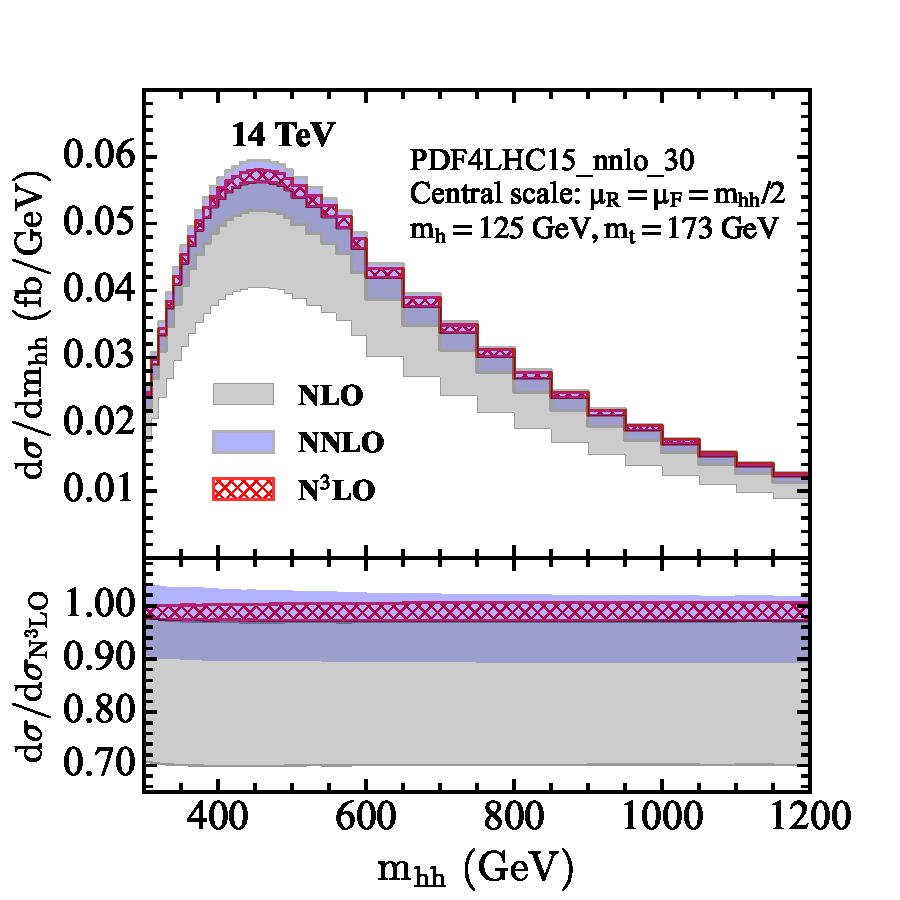
\includegraphics[width=0.49\textwidth]{N3LO_QCD_SM/N3LO_htl/Images/diff_large_mt_13_14_FO_CERNYR5}
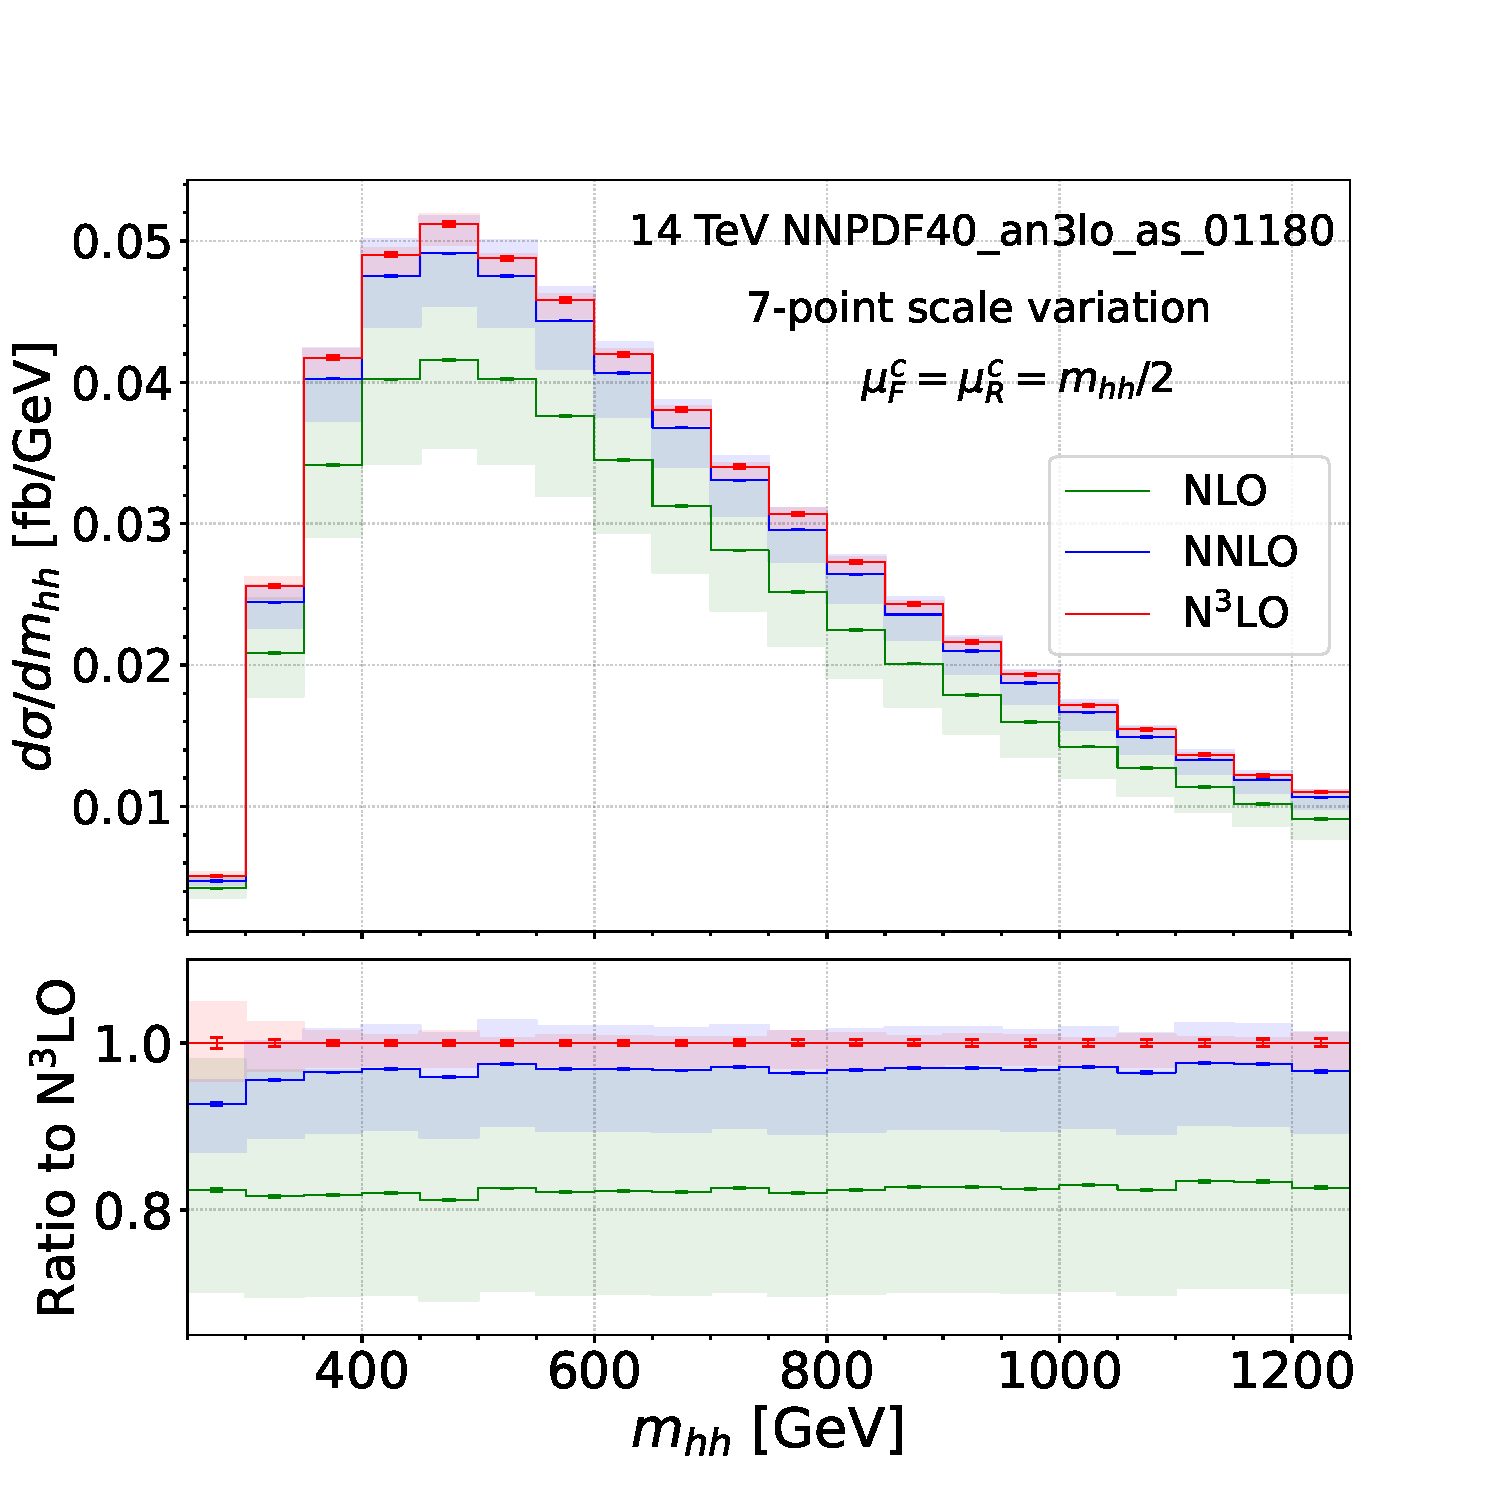
\includegraphics[width=0.49\textwidth,height=7.52cm]{N3LO_QCD_SM/N3LO_htl/Images/HH_m_hh}
\caption{Inclusive (left) and fiducial (right) invariant-mass distributions for Higgs boson pair production at $\sqrt{s}=14$ TeV in the HTL, from NLO to N$^3$LO. The error bands correspond to $7$-point scale variations. Here $\mu^C$ denotes the central value of the renormalization and factorization scales. Results shown are from Refs.~\cite{Chen:2019lzz,Chen:2019fhs,Chen:2026zmi}.}
\label{fig:xs_vs_mhh_FO_N3LO}
\end{figure*}


\begin{figure*}[ht]
\centering
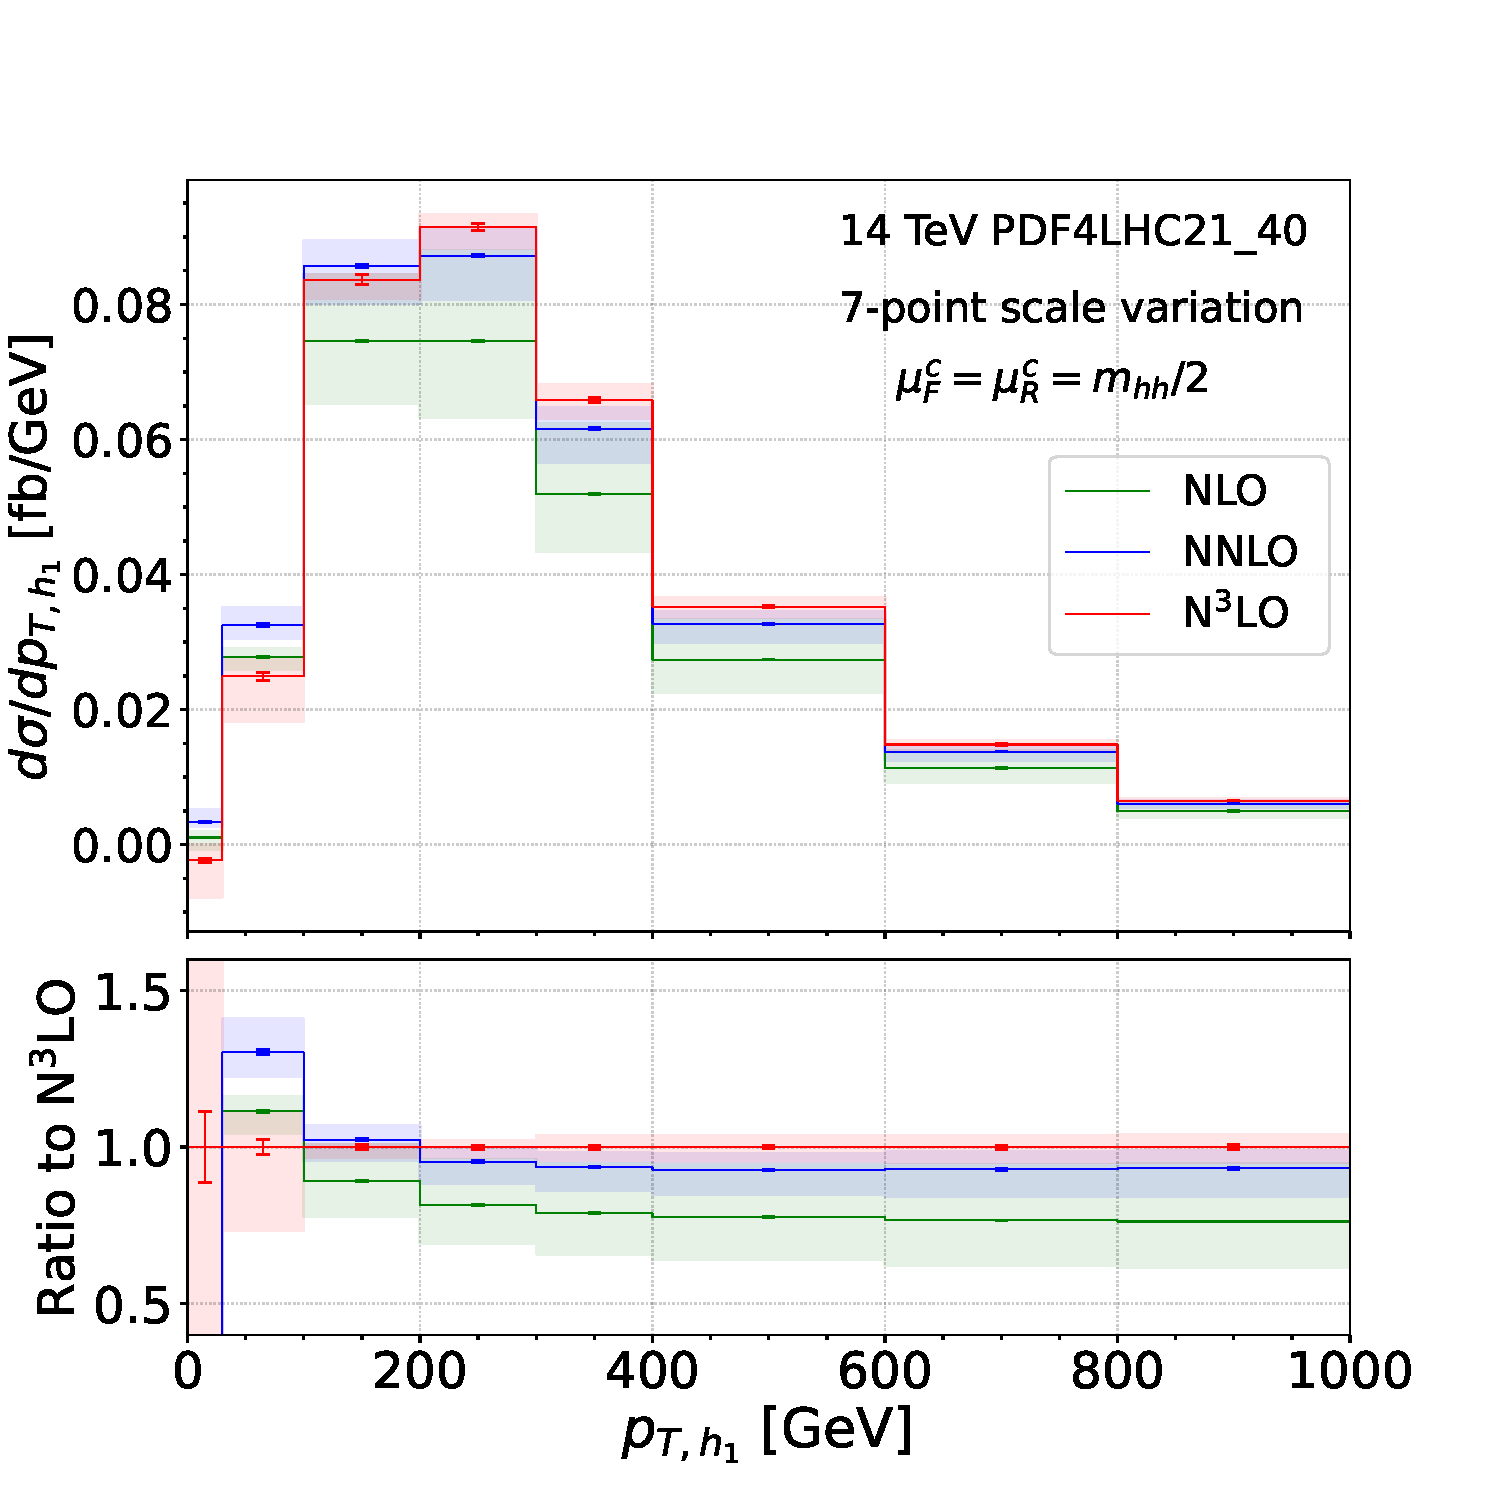
\includegraphics[width=0.49\textwidth,height=7.52cm]{N3LO_QCD_SM/N3LO_htl/Images/HH_pt_h1st_100.pdf}
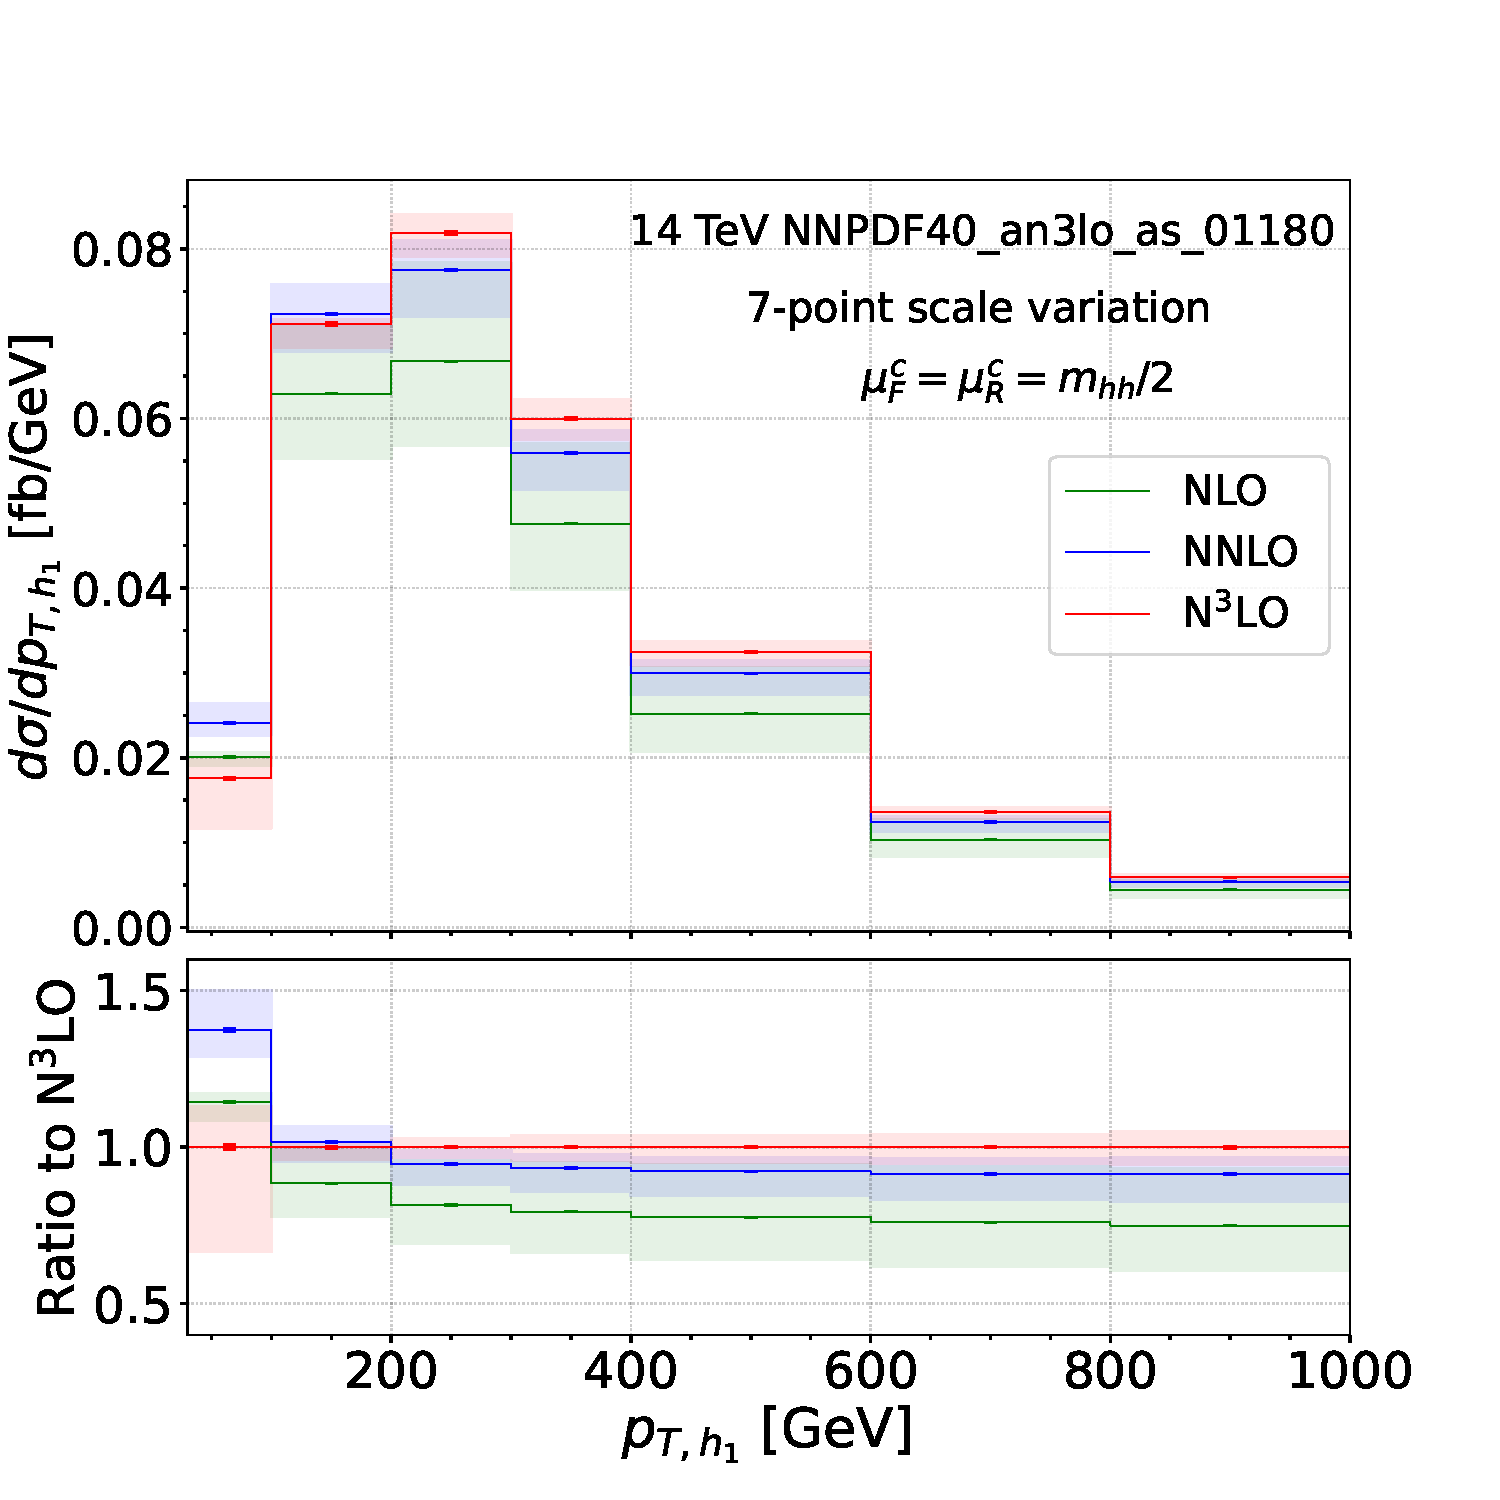
\includegraphics[width=0.49\textwidth,height=7.52cm]{N3LO_QCD_SM/N3LO_htl/Images/HH_pt_h1st.pdf}
\caption{Inclusive (left) and fiducial (right) leading-Higgs $p_{T}$ distributions for Higgs boson pair production at $\sqrt{s}=14$ TeV in the HTL, from NLO to N$^3$LO. The error bands correspond to $7$-point scale variations. Here $\mu^C$ denotes the central value of the renormalization and factorization scales. Results shown are from Ref.~\cite{Chen:2026zmi}.}
\label{fig:fid_pth1_FO_N3LO}
\end{figure*}


\begin{figure*}[ht]
\centering
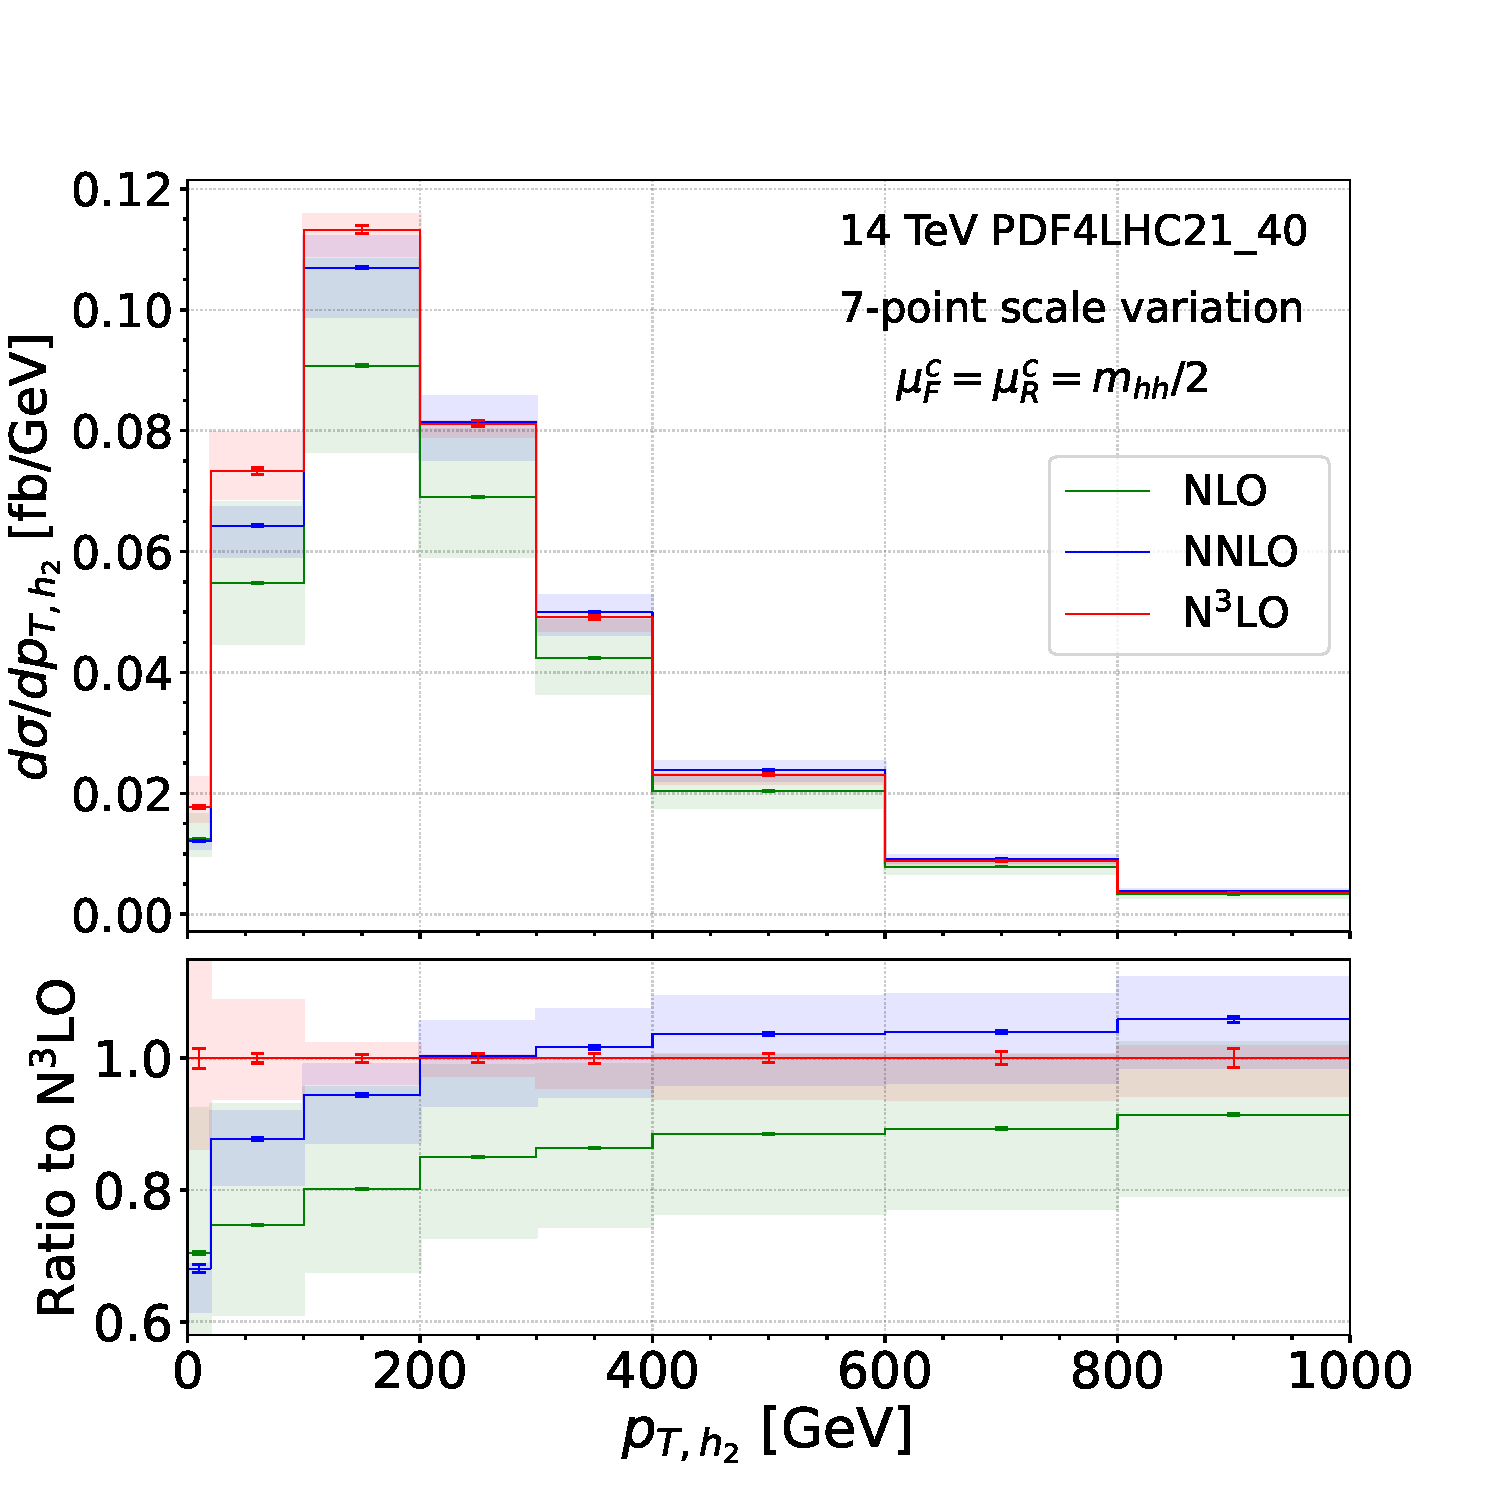
\includegraphics[width=0.49\textwidth,height=7.52cm]{N3LO_QCD_SM/N3LO_htl/Images/HH_pt_h2nd_100.pdf}
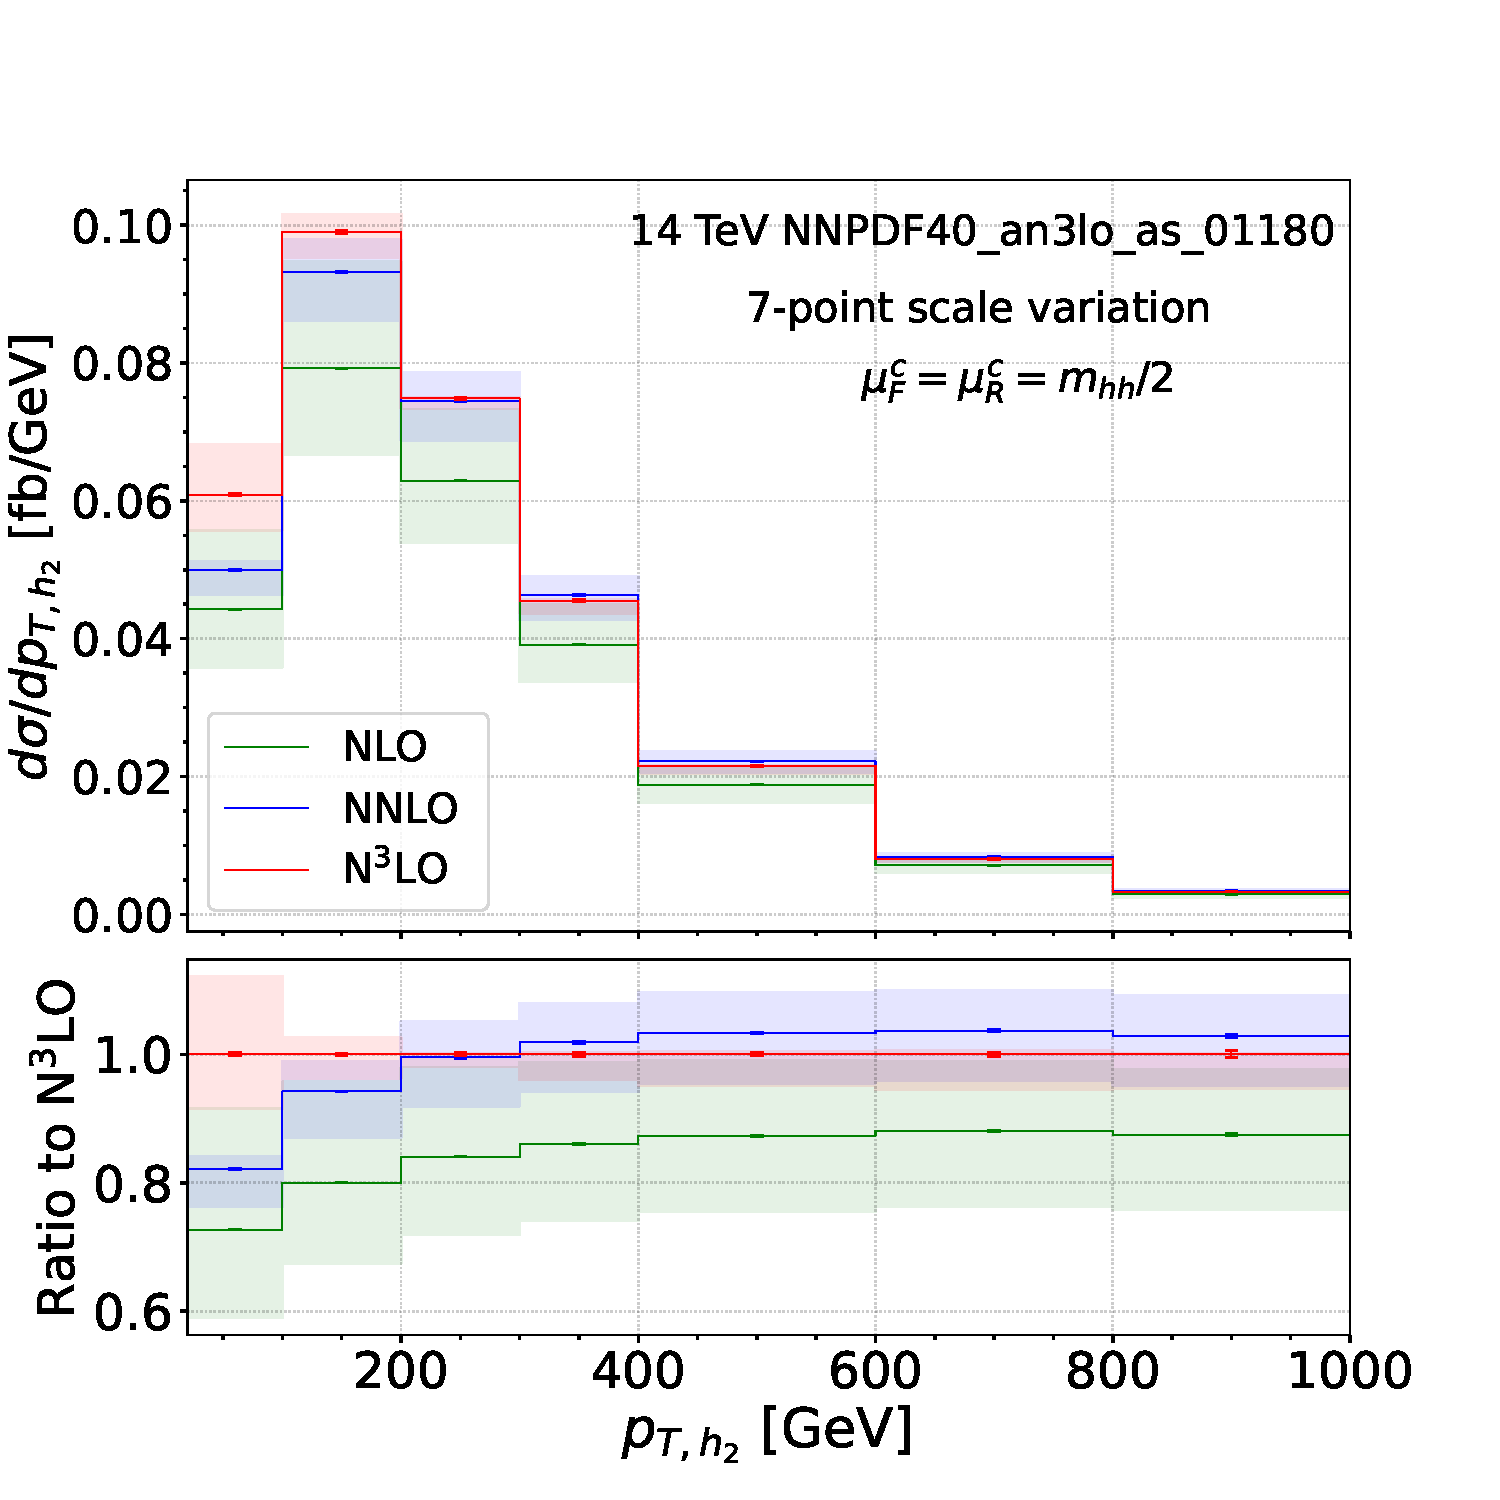
\includegraphics[width=0.49\textwidth,height=7.52cm]{N3LO_QCD_SM/N3LO_htl/Images/HH_pt_h2nd.pdf}
\caption{Inclusive (left) and fiducial (right) subleading-Higgs $p_{T}$ distributions for Higgs boson pair production at $\sqrt{s}=14$ TeV in the HTL, from NLO to N$^3$LO. The error bands correspond to $7$-point scale variations. Here $\mu^C$ denotes the central value of the renormalization and factorization scales. Results shown are from Ref.~\cite{Chen:2026zmi}.
}
\label{fig:fid_pth2_FO_N3LO}
\end{figure*}


The phase-space-integrated cross sections from NLO to N$^3$LO in the HTL at $\sqrt{s}=14$ TeV for proton-proton ($pp$) collisions are listed in Table~\ref{tab:FON3LOinclusivexs}. For the inclusive (fiducial) results, the N$^3$LO QCD corrections increase the NNLO cross section by $3\%$ ($4\%$) and reduce the fractional scale uncertainty by a factor of four (three).
The Higgs boson pair invariant-mass distributions at fixed orders in $\alpha_s$ are shown in Fig.~\ref{fig:xs_vs_mhh_FO_N3LO} for the inclusive (left panel) and fiducial (right panel) cases. In both cases, the higher-order QCD corrections do not shift the peak positions of the distributions. There is, however, a small difference between the two setups. In the inclusive case, the $K$-factor for N$^3$LO over NNLO is nearly flat across a wide range of $m_{hh}$, and the N$^3$LO prediction, with its small scale uncertainty, lies entirely within the NNLO uncertainty band. In contrast, with the fiducial cuts defined in Eq.~\eqref{eq:fiducialcuts}, the N$^3$LO correction in the first bin ($m_{hh}<300$ GeV) amounts to 8$\%$, which is almost a factor of two larger than the corrections in the other bins. Additionally, the scale uncertainty is significantly larger in this bin. The difference in the threshold region mainly stems from linear power corrections in the presence of fiducial cuts. The leading- and subleading-$p_T$ distributions of the two Higgs bosons are shown in Figs.~\ref{fig:fid_pth1_FO_N3LO} and~\ref{fig:fid_pth2_FO_N3LO}. The N$^3$LO QCD corrections modify their shapes, with the largest effects occurring in the small-$p_T$ region, where the scale uncertainties are also most significant. In this region, the fixed-order predictions are not stable, and a resummation calculation is necessary to stabilize the theoretical predictions. Moreover, the fiducial cuts also have a clear impact in this region. The scale uncertainty at N$^3$LO of $p_{T,h_1}$ ($p_{T,h_2}$) in the 20--100 GeV (30--100 GeV) bin changes from 38$\%$ (15$\%$) to 46$\%$ (21$\%$) after imposing the fiducial cuts.
In the intermediate- and large-$p_T$ regions, the fixed-order predictions remain reliable.


\subsection[\texorpdfstring{$\textup{N}^3\textup{LO} + \textup{N}^3\textup{LL}$ in the HTL}{N3LO + N3LL in the HTL}]{\texorpdfstring{\boldmath$\textup{N}^3\textup{LO} + \textup{N}^3\textup{LL}$ in the HTL}{N3LO + N3LL in the HTL}}

%\textit{Authors:} Ajjath A H, Hua-Sheng Shao (2209.03914)

\textbf{Ajjath A H, Hua-Sheng Shao~\cite{Ajjath:2022kpv}.}

\noindent Theoretical predictions for the Higgs boson pair production cross section can be further improved by resumming threshold logarithms from soft-gluon emissions. In this subsection, these logarithms are resummed to N$^3$LL accuracy~\cite{Ajjath:2022kpv}, following the formalism outlined briefly below.

Within the QCD-improved parton model, the differential cross section in the invariant mass squared $m_{hh}^2$
of the Higgs boson pair, for hadronic collisions at the centre-of-mass energy $\sqrt{s}$, can be written as a convolution of the partonic flux $\phi_{ab}$ and the perturbative coefficient function $\Delta_{ab\to hh}$
\begin{equation}\label{eq:partonmodel}
    m_{hh}^2 \dfrac{d}{d m_{hh}^2}\sigma_{pp\rightarrow hh}(s,m_{hh}^2) = \tau \sum_{a,b=q,\bar q,g} \int_\tau^1 \frac{dz}{z} \phi_{ab}\left(\frac{\tau}{z},\mu_F^2\right)~ \Delta_{ab\rightarrow hh}  \left(z,m_{hh}^2,\mu_F^2\right)\,,
\end{equation}
where $\tau\equiv m_{hh}^2/s$, $z\equiv m_{hh}^2/\hat{s}$, with $\sqrt{\hat{s}}$
the partonic centre-of-mass energy.

 In the threshold limit, $z\rightarrow1$, the dominant (leading-power, LP) terms arise from both virtual loop corrections and soft, unresolved real-gluon emissions. These contributions take the form of Dirac delta functions, $\delta(1-z)$,  and plus-distributions, such as $ {\cal D}_k(z) \equiv  \left(\frac{\ln^k{(1-z)}}{1-z}\right)_+$, reflecting the incomplete cancellation between virtual and real radiation associated with soft-gluon emissions. These singular threshold contributions can be systematically factorized as
\begin{align}\label{eq:partonicxsec}
    \Delta^{\text{LP}}_{gg\rightarrow hh}(z,m_{hh}^2,\mu_F^2) =& H_{gg\rightarrow hh}(m_{hh}^2,\mu_R^2) ~\delta(1-z)\otimes S_{\Gamma,gg}(z,m_{hh}^2,\mu_F^2,\mu_R^2)\,,
\end{align}
where $H_{gg\rightarrow hh}$ encodes the process-dependent hard virtual corrections after infrared-divergence subtraction, and
 $S_{\Gamma,gg}$
  is the soft-collinear function describing gluon emissions that are soft, collinear, or both with respect to the parent partons. Singular terms are retained in this factorization, while power-suppressed corrections in $(1-z)$ are neglected. The threshold-enhanced logarithms resummed in this approach are universal and can largely be expressed in terms of process-independent anomalous dimensions and splitting functions. Detailed structures of these functions are given in Refs.~\cite{Ravindran:2005vv,Ahmed:2020nci,Ajjath:2022kpv}.

The universal nature of the soft and collinear terms allows the resummation of large logarithms to all orders in $\alpha_s$ using renormalization group methods. This resummation is efficiently performed in Mellin $N$-moment space, where the threshold limit $z\rightarrow 1$ corresponds to $N\rightarrow \infty$:
\begin{align}
    \Delta_{gg\rightarrow hh}^{\rm res}(N,m_{hh}^2,\mu_F^2) =&  \int_0^1 dz ~z^{N-1}\Delta^{\text{LP}}_{gg\rightarrow hh}\left(z,m_{hh}^2,\mu_F^2\right)
    \nonumber \\
    =  g_{0,gg\to hh}(m_{hh}^2,\mu_F^2,\mu_R^2)
    & 
    ~\exp \left(\tilde{C}_{0,gg} (a_s(\mu_R^2)) + g_{1,gg} (\omega)\ln N + \sum_{k=2}{a_s^{k-2}(\mu_R^2)~g_{k,gg} (\omega)}\right)\,,
    \label{DeltaN}
\end{align}
where $a_s\equiv \alpha_s/4\pi$ and $\omega \equiv 2 \beta_0 a_s(\mu_R^2) \ln N$. The factor $g_{0,gg\to hh}$, outside the exponent, arises from the $N$-independent hard function and the Altarelli-Parisi splitting kernels, while the functions $g_{k,gg}$, $k\ge 1$, encode the resummation of logarithmic contributions up to the specified logarithmic accuracy (LL, NLL, NNLL, N$^3$LL, etc.).
Furthermore, the exponent contains an additional $N$-independent coefficient, $\tilde{C}_{0,gg}$, arising from the ${\cal O}(1)$ terms of ${\cal D}_k(z)$ after the Mellin transform; it depends on the Riemann zeta functions $\zeta_n$ and the Euler-Mascheroni constant $\gamma_E$. 

The structure above ensures that the resummation captures all LP threshold logarithms at each order, resulting in a perturbative series with greatly improved convergence and reduced dependence on the renormalization and factorization scales. Matching to fixed-order calculations guarantees the exact reproduction of known results and prevents double counting of terms already included at a given order. At the $\NkLONkLL$ accuracy, the double counting corresponds to $\Delta^{\text{LP}}_{gg\to hh}$ expanded up to N$^k$LO in $\alpha_s$. However, at a given logarithmic accuracy, the right-hand side of the resummation formalism in Eq.~\eqref{DeltaN} is not uniquely defined. The assignment of $N$-independent terms inside or outside the exponent introduces a degree of arbitrariness, referred to as the resummation scheme dependence~\cite{Ajjath:2022kpv}. Four different resummation schemes, denoted ${\rm N_1}$, $\rm{\overline N}_1$, ${\rm N_2}$, and $\rm{\overline N}_2$, are considered in Ref.~\cite{Ajjath:2022kpv} (see their definitions in Section 2.4 of that reference).

A comparison of inclusive Higgs boson pair cross sections at $\sqrt{s}=14$ TeV in the HTL, at several perturbative orders and in different resummation schemes, is shown in Fig.~\ref{fig:Verical_prescription}. Both the fixed-order N$^k$LO and resummation-improved N$^k$LO+N$^k$LL predictions are presented, with error bars indicating scale uncertainties. We stress a few key points:
\begin{itemize}
    \item Although a significant resummation scheme dependence is observed at NLO+NLL, this dependence decreases as higher orders are included and becomes moderate at N$^3$LO+N$^3$LL.
    \item The results in the $\ResNTwo$ and $\ResNbTwo$ schemes show faster perturbative convergence than those in the other two schemes.
    \item The inclusion of threshold resummation further reduces scale uncertainties. For instance, in the $\ResNbTwo$ scheme, the N$^3$LO+N$^3$LL scale-uncertainty band is reduced by a factor of two compared to the N$^3$LO result, and nearly by a factor of four compared to the NNLO+NNLL result in the same scheme.
    \item The resummation scheme uncertainty at N$^3$LO+N$^3$LL is subdominant compared to the residual scale uncertainty. At $14$ TeV, for example, we have \begin{equation*}\sigma_{\rm N^3LO+N^3LL}=38.70\left(^{+0.85\%}_{-0.87\%}\right)_{\rm scale}\left(^{+0.08\%}_{-0.39\%}\right)_{\rm scheme}~\mathrm{fb}.
    \end{equation*}
\end{itemize}
Therefore, in the following, we consider the $\ResNbTwo$ scheme only. Table~\ref{tab:ResumN3LON3LLinclusivexs} summarizes inclusive cross sections, from NLO+NLL to N$^3$LO+N$^3$LL, in the HTL at $\sqrt{s}=14$ TeV. Inclusion of N$^3$LL resummation corrections increases the N$^3$LO cross section by around $1\%$ and reduces the scale uncertainty by about a factor of two.


\begin{figure*}[ht]
\centering
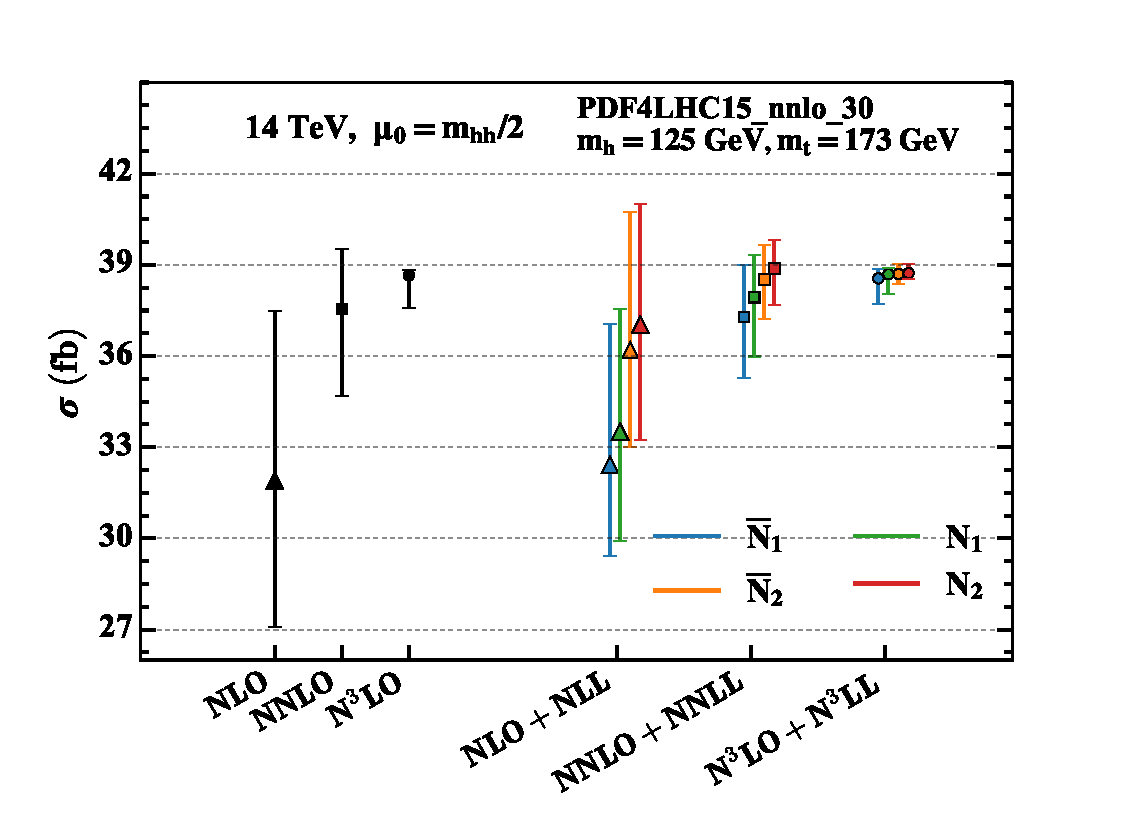
\includegraphics[width=0.5\textwidth]{N3LO_QCD_SM/N3LO_N3LL/Images/prescription_14TeV_YR5.pdf}
\caption{Inclusive Higgs boson pair cross sections at $\sqrt{s}=14~\textup{TeV}$ in the HTL at several perturbative orders and in different resummation schemes. The error bars indicate scale uncertainties. Results shown are from Ref.~\cite{Ajjath:2022kpv}.}
\label{fig:Verical_prescription}
\end{figure*}

\begin{table}[htbp] 
\begin{center}
\newcolumntype{P}[1]{>{\centering\arraybackslash}p{#1}}
{\renewcommand{\arraystretch}{1.5}
%\begin{tabular}{|P{2.5cm}|P{2.5cm}|P{2.5cm}|}
\begin{tabular}{P{2.6cm}P{2.6cm}P{2.6cm}}
%\hline
    \toprule
    $\sigma_{\textup{NLO}+\textup{NLL}}$ $[\textup{fb}]$
    & $\sigma_{\textup{NNLO}+\textup{NNLL}}$ $[\textup{fb}]$
    & $\sigma_{\textup{N}^3\textup{LO}+\textup{N}^3\textup{LL}}$ $[\textup{fb}]$
    \\
%  \hline
    \midrule
  $36.19^{+12.5\%}_{-8.8\%}$ &
  $38.52^{+3.0\%}_{-3.4\%}$ &
 $38.70_{-0.85\%}^{+0.87\%}$
 \\
% \hline
    \bottomrule
\end{tabular}}
%\end{small}
\caption{Soft-gluon resummation–improved inclusive cross sections in the HTL at $\sqrt{s}=14~\textup{TeV}$. The quoted uncertainties correspond to $7$-point scale variations. Only results in the $\ResNbTwo$ scheme are shown.}
\label{tab:ResumN3LON3LLinclusivexs}
\end{center}
\end{table}

\begin{figure*}[!htbp]
\centering
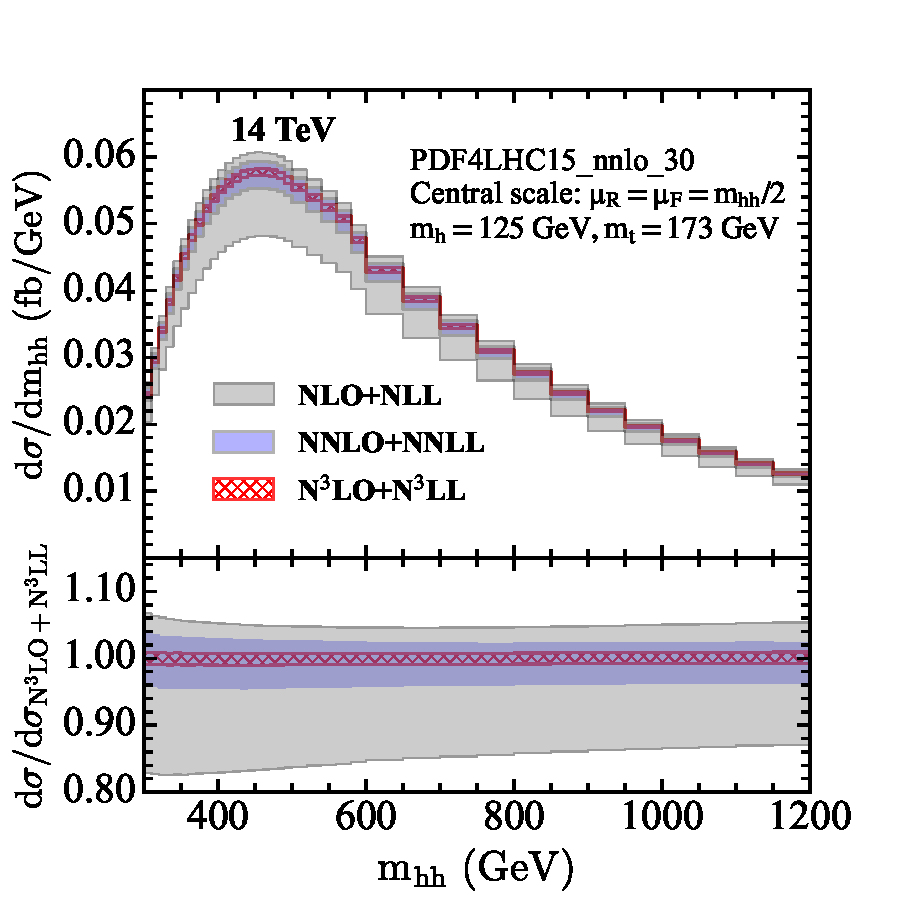
\includegraphics[width=0.5\textwidth]{N3LO_QCD_SM/N3LO_N3LL/Images/diff_large_mt_13_14_resum_CERNYR5.pdf}
\\
\caption{Inclusive invariant-mass distributions for Higgs boson pair production at $\sqrt{s}=14$ TeV in the HTL, from NLO+NLL to N$^3$LO+N$^3$LL. The error bands correspond to $7$-point scale variations. Results shown are from Ref.~\cite{Ajjath:2022kpv}.}
\label{fig:xs_vs_mhh_Res_N3LON3LL}
\end{figure*}

The differential prediction for the Higgs boson pair invariant mass $m_{hh}$ in Fig.~\ref{fig:xs_vs_mhh_Res_N3LON3LL} further demonstrates the perturbative convergence of the strong-coupling expansion. Soft-gluon resummation induces only a modest shift in the spectrum and further reduces the fractional scale errors.


\subsection{Including partial top quark mass effects}

%\textit{Authors:} Ajjath A H, Long-Bin Chen, Hai Tao Li, Hua-Sheng Shao, Jian Wang (1912.13001, 2209.03914)

\textbf{Ajjath A H, Long-Bin Chen, Xuan Chen, Yuesheng Dai, Hai Tao Li, Shi-Yuan Li, Hua-Sheng Shao, Jian Wang~\cite{Chen:2019fhs,Ajjath:2022kpv,Chen:2026zmi}.}

\noindent Since finite top quark mass effects cannot be neglected and are exactly known only at NLO~\cite{Borowka:2016ehy,Borowka:2016ypz,Baglio:2018lrj,Davies:2019dfy}, we improve the NLO QCD computation with full top quark mass dependence~\cite{Heinrich:2017kxx,Heinrich:2019bkc,Davies:2025qjr} (denoted as ``$\NLOmt$") by multiplying it with the higher-order (differential) $K$-factors calculated in the HTL in this subsection. The reweighting is carried out consistently using the on-shell top quark mass scheme in $\NLOmt$ and the on-shell mass in the HTL predictions. The resulting combinations are denoted as $\NkLOtimesNLOmt$ and $\NkLONkLLtimesNLOmt$, where $k$ is a positive integer. Specifically,
\begin{eqnarray}\label{NkLO-fullmt}
d\sigma_{\NkLOtimesNLOmt}&\equiv& d\sigma_{\NLOmt}\frac{d\sigma_{\NkLO}}{d\sigma_{\rm NLO}}\,,\nonumber\\
d\sigma_{\NkLONkLLtimesNLOmt}&\equiv&d\sigma_{\NLOmt}\frac{d\sigma_{\NkLONkLL}}{d\sigma_{\rm NLO}}\,.
\end{eqnarray}
This treatment is justified under certain working assumptions; alternative approaches to incorporating top quark mass effects can be found in Section~3 of Ref.~\cite{Chen:2019fhs}.




\begin{sloppypar}
The inclusive phase-space-integrated cross sections are listed in Table~\ref{Tab:fullMt_inc} for LHC $pp$ collisions at $\sqrt{s}=14$ TeV and for five perturbative orders: $\NLOmt$, $\NNLOtimesNLOmt$, $\NNLONNLLtimesNLOmt$, $\NtLOtimesNLOmt$, and $\NtLONtLLtimesNLOmt$. The N$^3$LO QCD corrections enhance the $\NLOmt$ cross section by $21\%$. The N$^3$LL threshold resummation only marginally modifies the $\NtLOtimesNLOmt$ cross section. The scale uncertainty is significantly reduced when higher-order QCD corrections are included: the width of the uncertainty band from the envelope of the $7$-point scale variation in $\NtLOtimesNLOmt$ is only about one quarter of that in the previous fixed-order $\NNLOtimesNLOmt$ result. Inclusion of N$^3$LL threshold resummation further reduces the scale uncertainty to below one percent. A similar pattern is observed in the differential invariant-mass distribution of the Higgs boson pair, as shown in the left panel of Fig.~\ref{fig:xs_vs_mhh_large_mt1}.
\end{sloppypar}

With the fiducial cuts defined in Eq.~\eqref{eq:fiducialcuts}, only fixed-order predictions are given in Table~\ref{Tab:fullMt_inc}, as fully differential soft-gluon resummation predictions are not available. The N$^3$LO QCD corrections enhance the $\NLOmt$ cross section by $18\%$, which is close to the inclusive case. The $m_{hh}$ distribution with fiducial cuts, shown in the right panel of Fig.~\ref{fig:xs_vs_mhh_large_mt1}, highlights the necessity of including finite top quark mass effects. A similar behaviour is seen in the $p_T$ distributions of the leading and subleading Higgs bosons in Figs.~\ref{fig:fid_pth1_mt} and~\ref{fig:fid_pth2_mt}. For more detailed discussions, we refer the interested reader to Ref.~\cite{Chen:2026zmi}.



\begin{table}%[ht] 
\begin{center}

% \begin{small}
\newcolumntype{P}[1]{>{\centering\arraybackslash}m{#1}}
{\renewcommand{\arraystretch}{1.5}
%\begin{tabular}{|P{4cm}|P{3cm}|}
\resizebox{0.98\textwidth}{!}{%
\begin{tabular}{P{5cm}P{5cm}P{5cm}}
%\hline
    \toprule
        Contributions   &Inclusive cross section [$\textup{fb}$]  &Fiducial cross section [$\textup{fb}$] \\
    \midrule
%    $\sigma_{\NLOmt}$ & $32.64_{-12.5\%}^{+13.5\%}~\textup{fb}$\\
    $\NLOmt$ & $32.64_{-12.5\%}^{+13.5\%}$  &  $28.44_{-12 \%}^{+14 \%}$ \\
%     \hline
%    $\sigma_{\NNLOtimesNLOmt}$ & $38.42_{-7.6\%}^{+5.2\%}~\textup{fb}$\\
    $\NNLOtimesNLOmt$ & $38.42_{-7.6\%}^{+5.2\%}$ & $33.40_{-7.3 \%}^{+5.2 \%}$ \\
%    \hline
%   $\sigma_{\NNLONNLLtimesNLOmt}$ & $39.42_{-3.4\%}^{+3.0\%}~\textup{fb}$    \\
   $\NNLONNLLtimesNLOmt$ & $39.42_{-3.4\%}^{+3.0\%}$  & -  \\
%    \hline
%    $\sigma_{\NtLOtimesNLOmt}$ & $39.56_{-2.7\%}^{+0.50\%}~\textup{fb}$ \\  
    $\NtLOtimesNLOmt$ & $39.56_{-2.7\%}^{+0.50\%}$ & $34.68(4)^{+1.4\%}_{-2.9\%}$ \\  
%    \hline
%    $\sigma_{\NtLONtLLtimesNLOmt}$ &  $39.60_{-0.87\%}^{+0.85\%}~\textup{fb}$ \\
    $\NtLONtLLtimesNLOmt$ &  $39.60_{-0.87\%}^{+0.85\%}$ & - \\
% \hline
%  \hline
    \bottomrule
\end{tabular}}}
\caption{Inclusive and fiducial phase-space-integrated cross sections for Higgs boson pair production via gluon fusion at $\sqrt{s}=14\,\textup{TeV}$ in $pp$ collisions, including top quark mass effects. The quoted relative uncertainties correspond to $7$-point scale variations.}
\label{Tab:fullMt_inc}
\end{center}
\end{table}

\begin{figure*}[!htbp]
\centering
\vspace{-1.5cm}
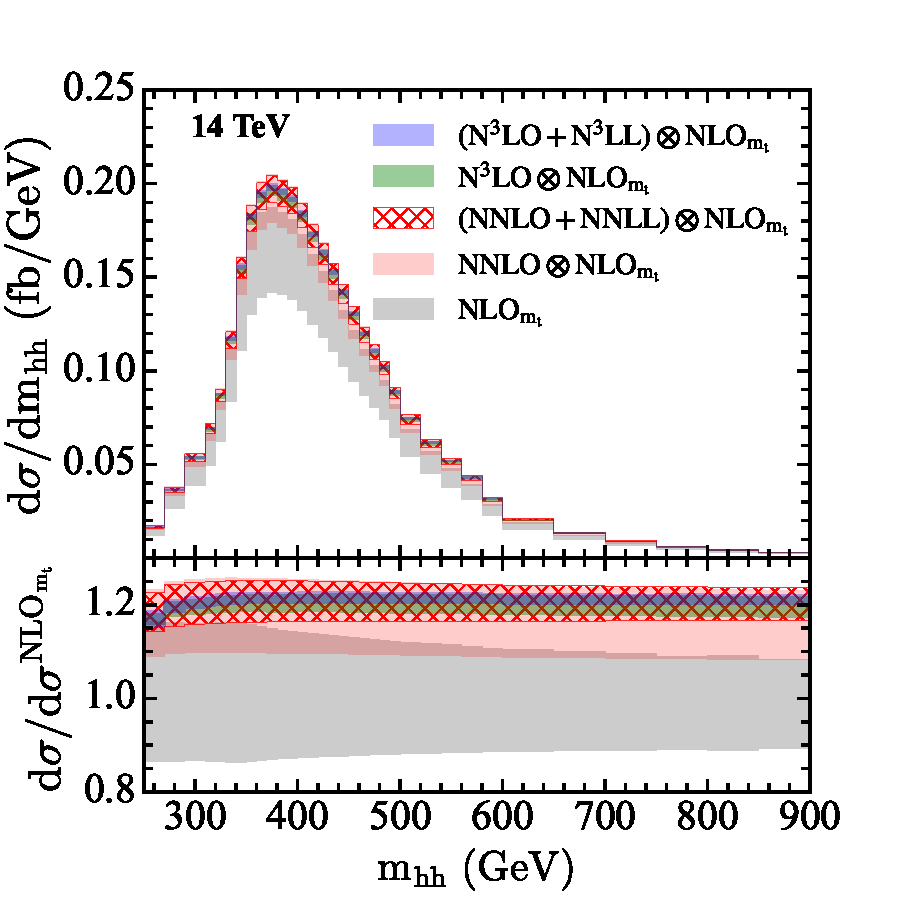
\includegraphics[width=0.49\textwidth]{N3LO_QCD_SM/N3LO_mt/Images/diff_full_mt_13_14_CERNYR5}
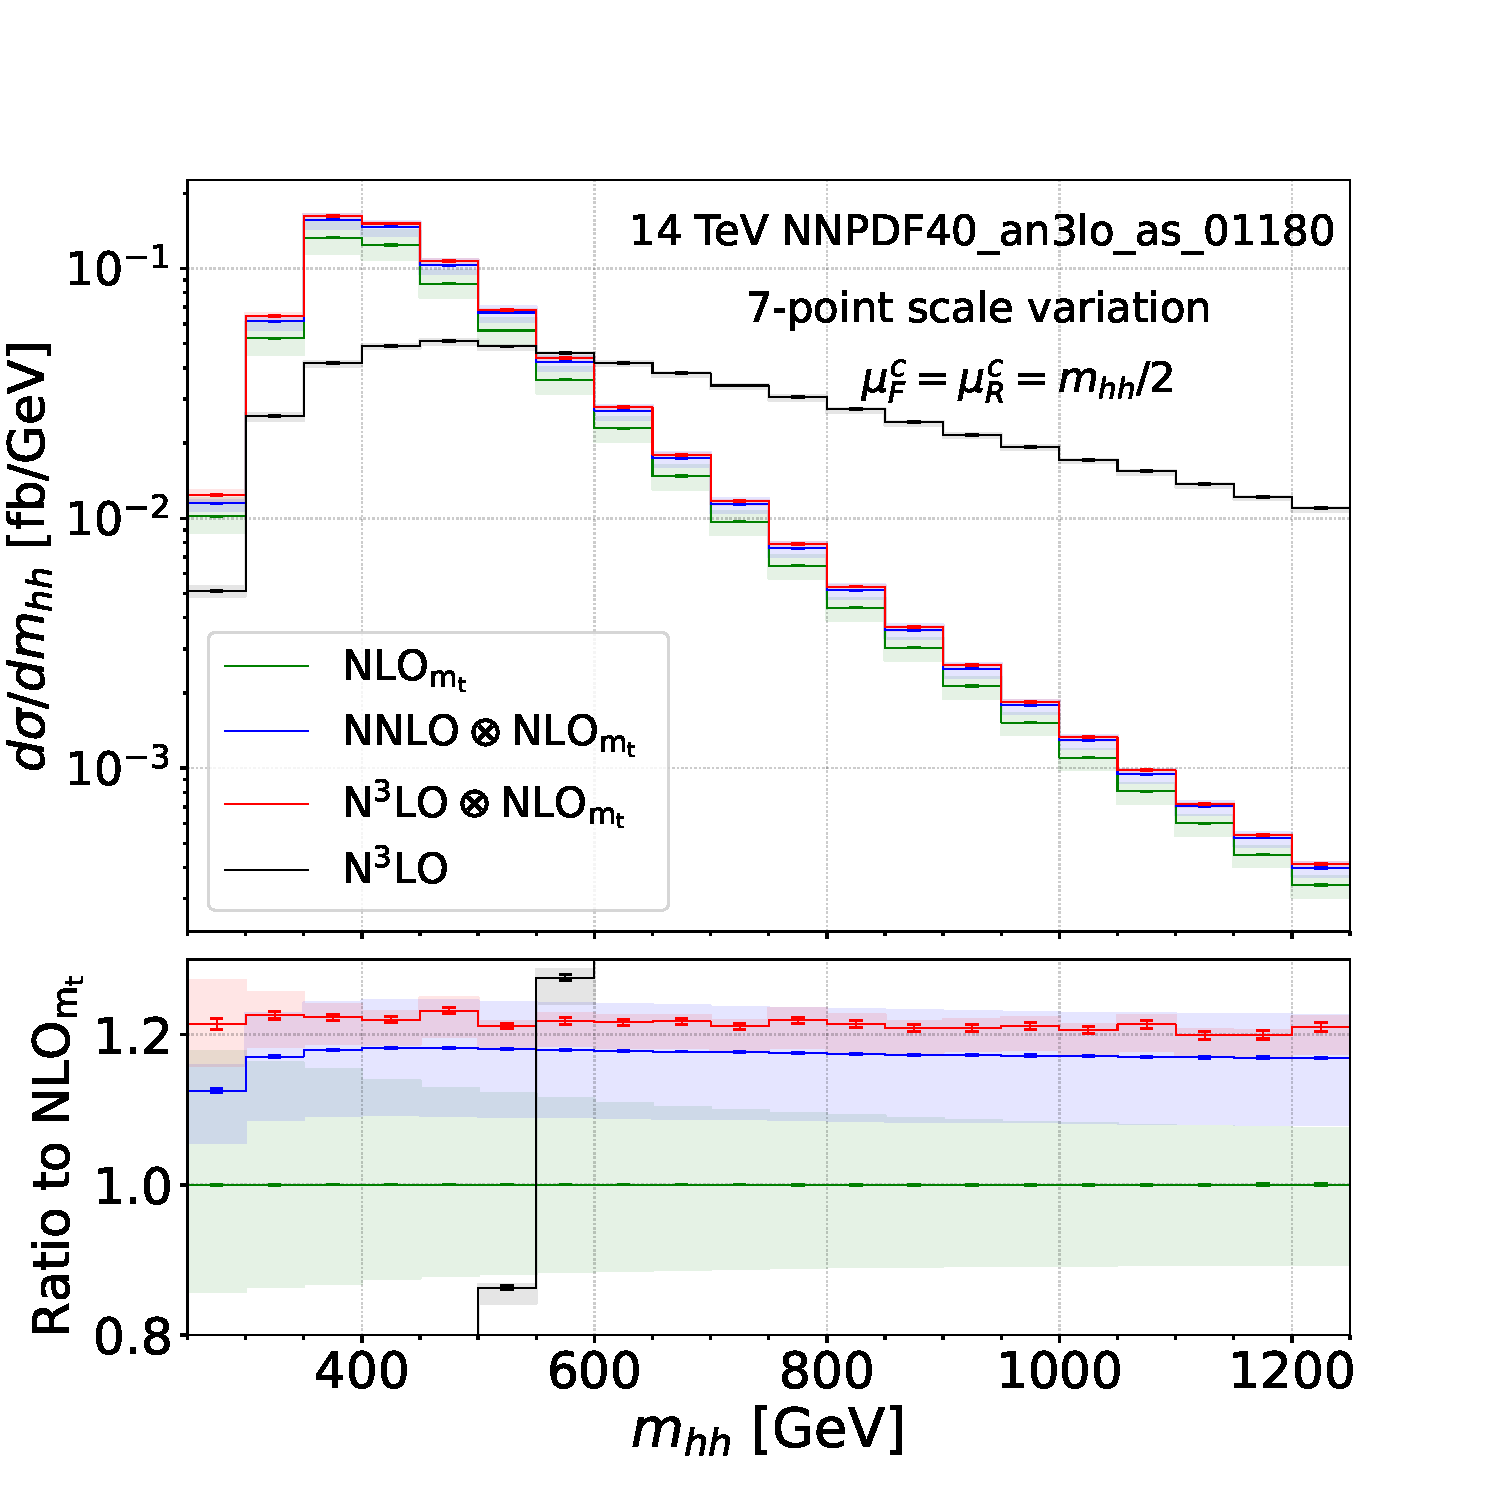
\includegraphics[width=0.49\textwidth,height=7.52cm]{N3LO_QCD_SM/N3LO_mt/Images/HH_m_hh_r}
\\
\caption{Inclusive (left) and fiducial (right) invariant-mass distributions for Higgs boson pair production at $\sqrt{s}=14$ TeV, including top quark mass effects. The error bands stem from $7$-point scale variations. Here $\mu^C$ denotes the central value of the renormalization and factorization scales. Results shown are from Refs.~\cite{Chen:2019fhs,Ajjath:2022kpv,Chen:2026zmi}.}
\label{fig:xs_vs_mhh_large_mt1}
\end{figure*}



\begin{figure*}[h]
\centering
\vspace{-2cm}
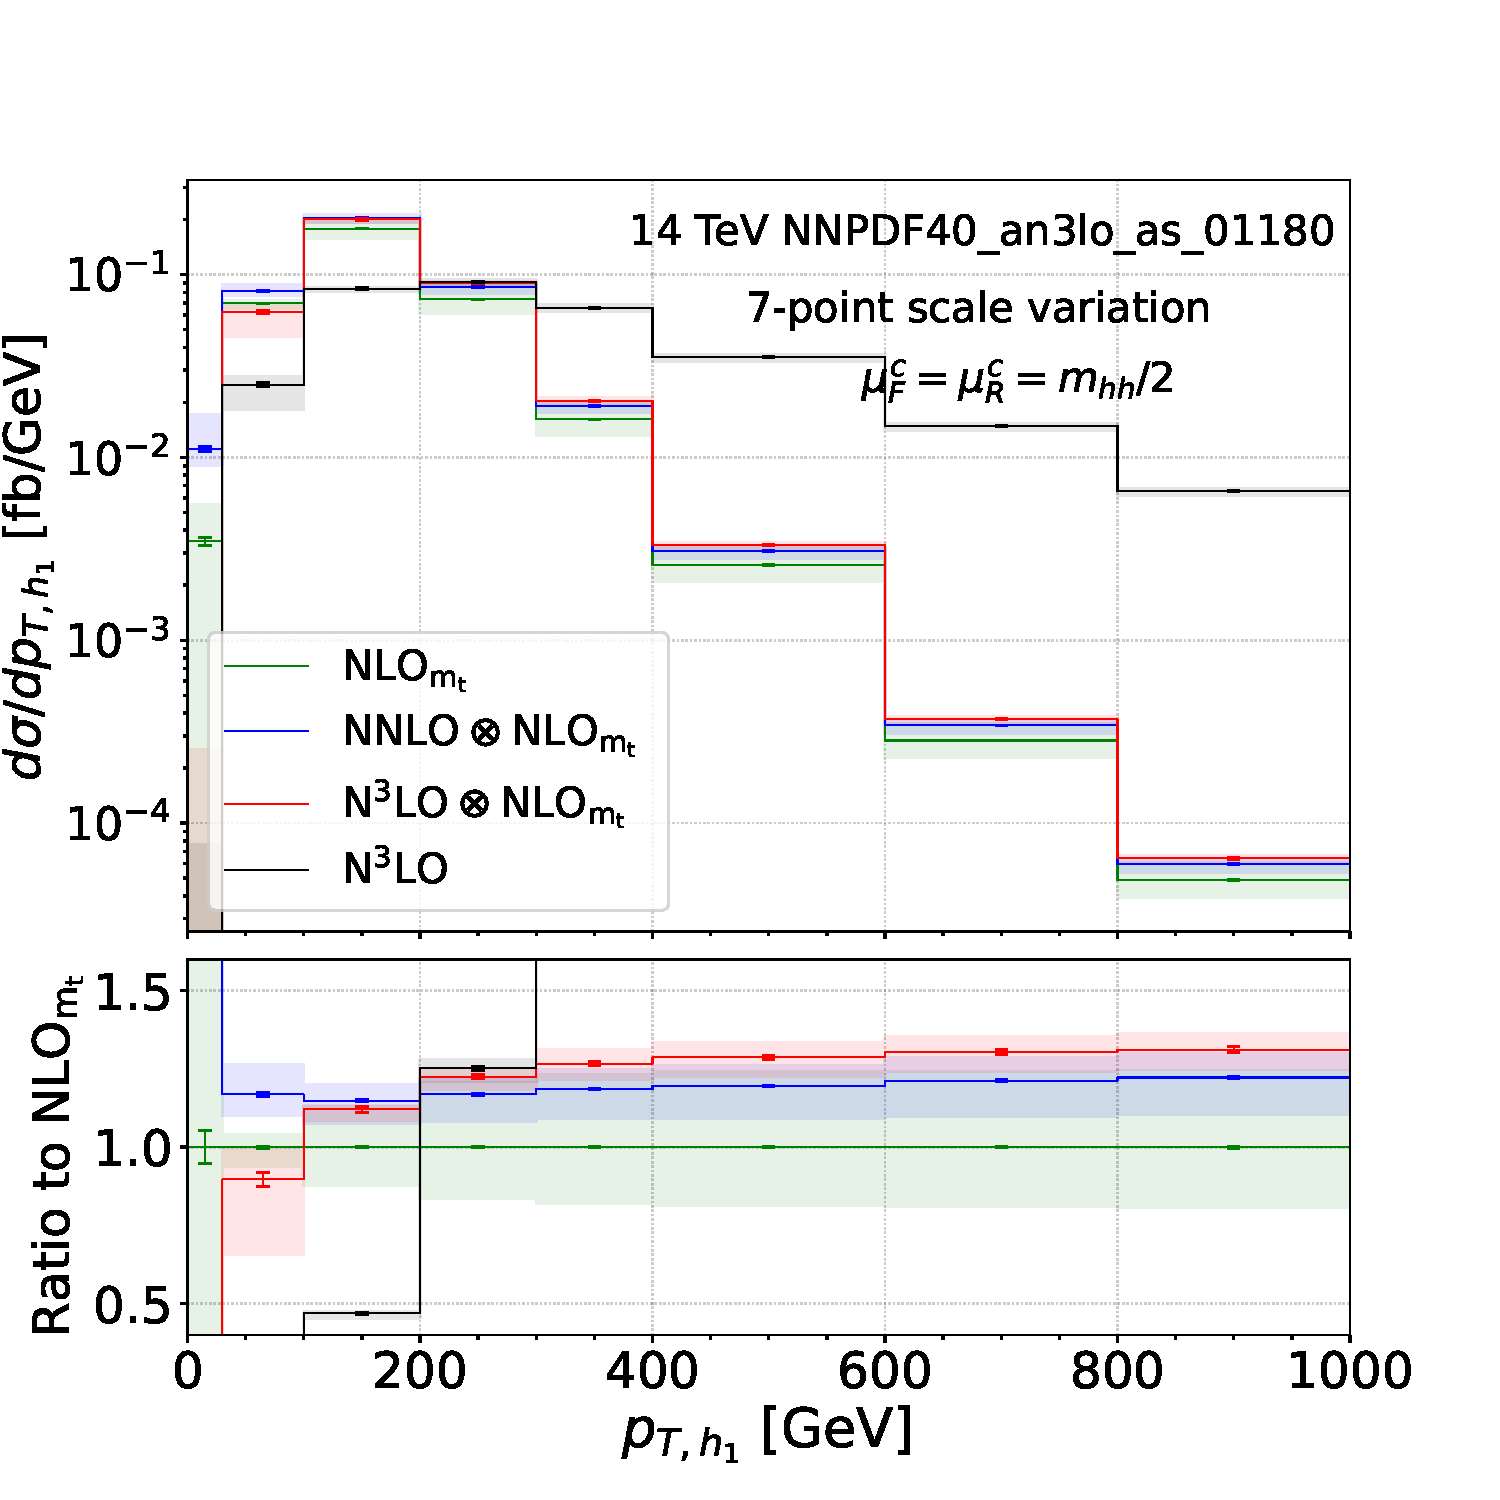
\includegraphics[width=0.49\textwidth,height=7.52cm]{N3LO_QCD_SM/N3LO_mt/Images/HH_pt_h1st_100_r.pdf}
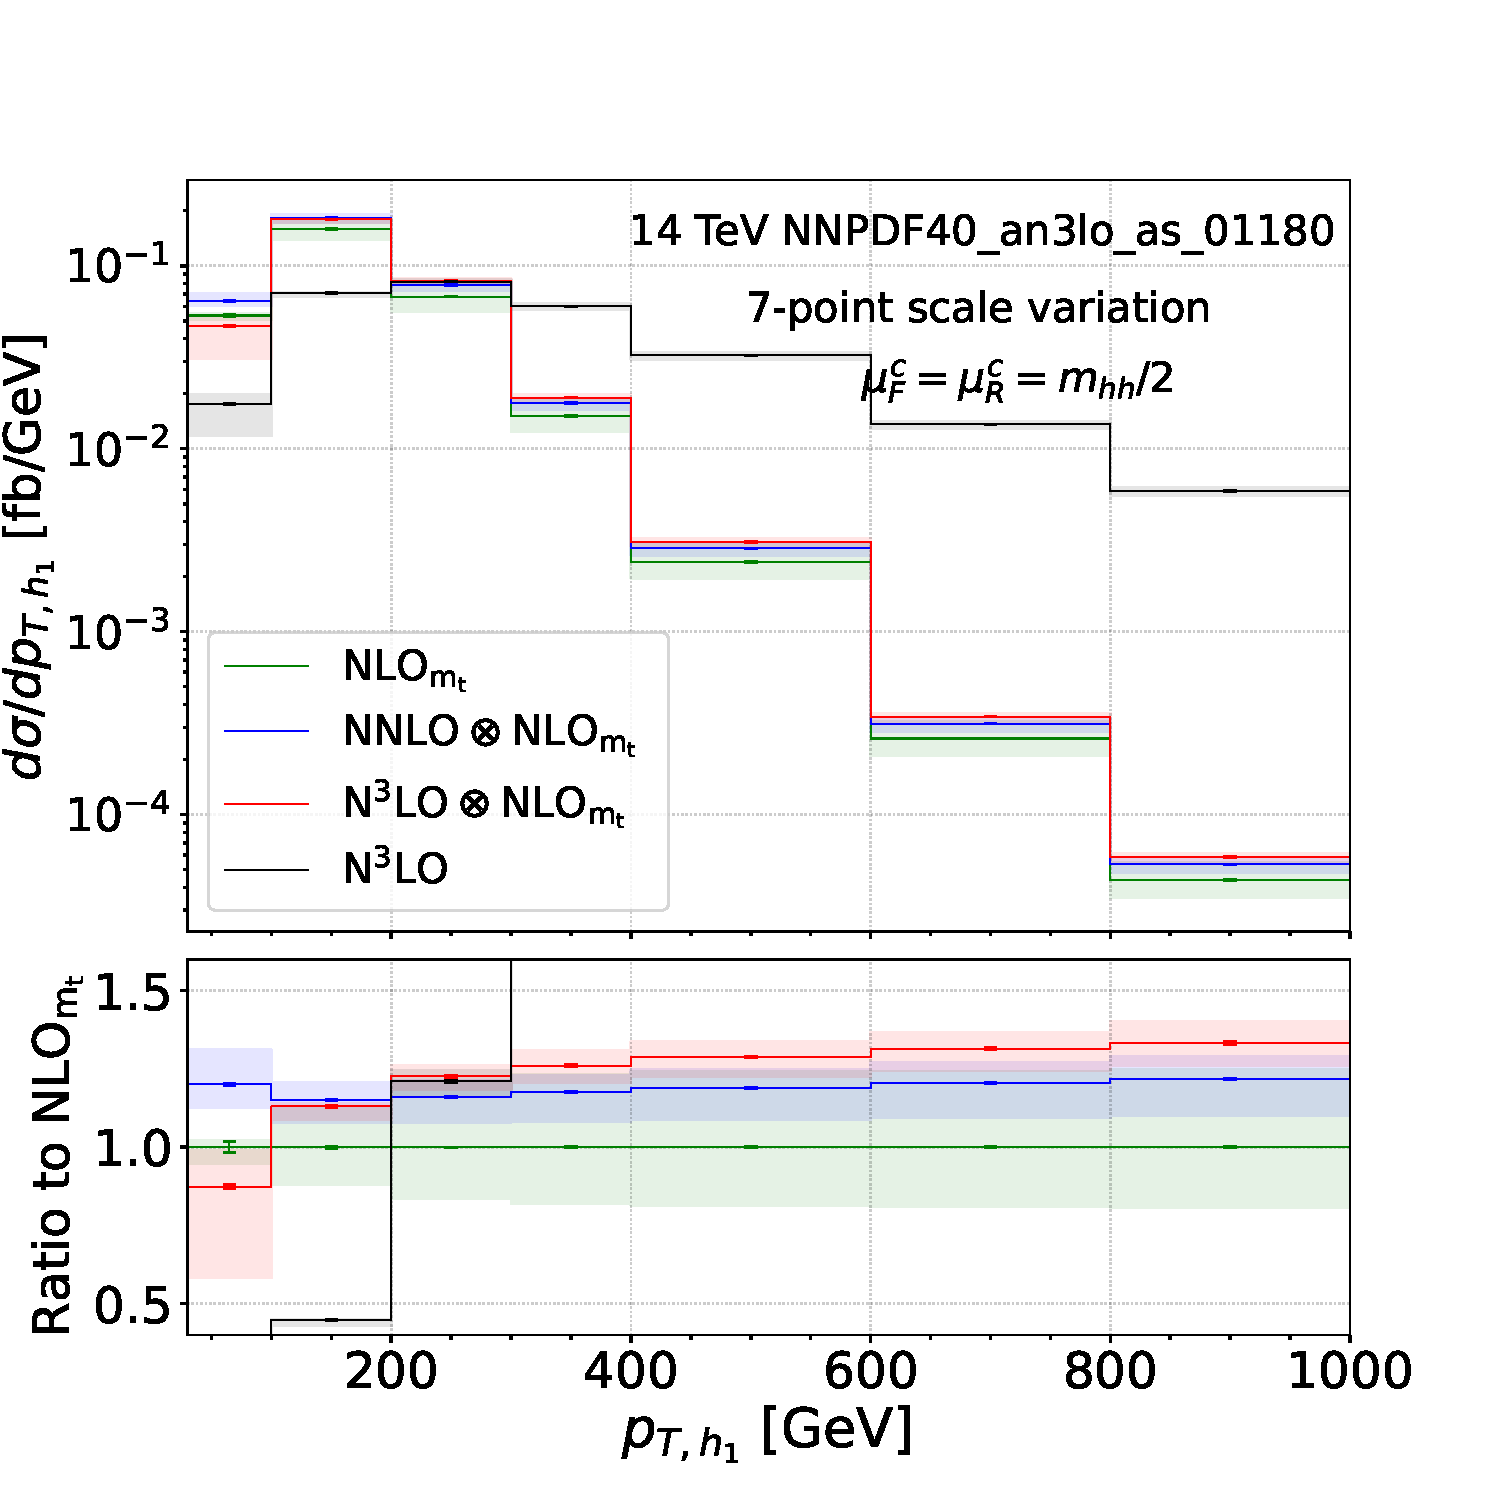
\includegraphics[width=0.49\textwidth,height=7.52cm]{N3LO_QCD_SM/N3LO_mt/Images/HH_pt_h1st_r.pdf}
\caption{Inclusive (left) and fiducial (right) leading-Higgs $p_{T}$ distributions for Higgs boson pair production at $\sqrt{s}=14$ TeV, including top quark mass effects. The error bands stem from $7$-point scale variations. Here $\mu^C$ denotes the central value of the renormalization and factorization scales. Results shown are from Ref.~\cite{Chen:2026zmi}.}
\label{fig:fid_pth1_mt}
\end{figure*}


\begin{figure*}[h]
\centering
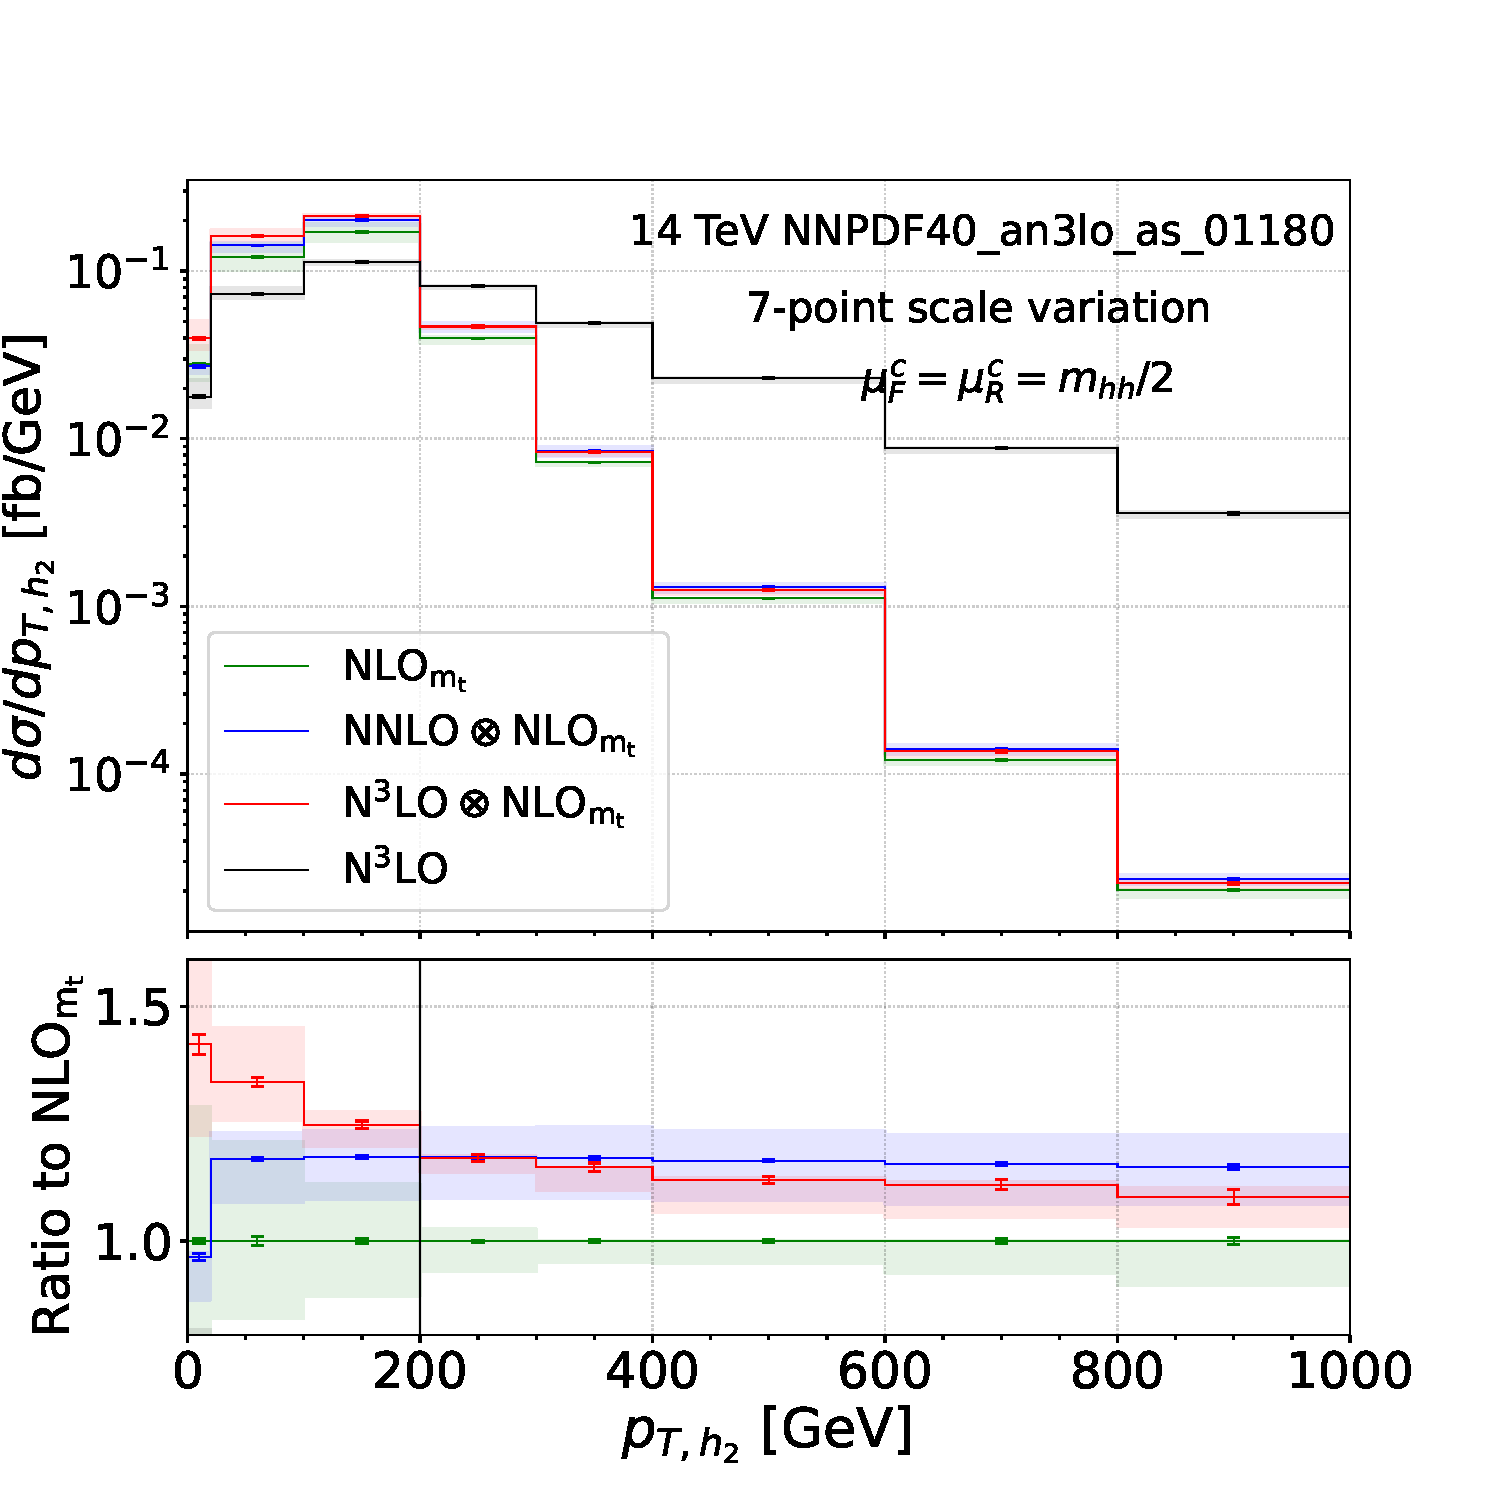
\includegraphics[width=0.49\textwidth,height=7.52cm]{N3LO_QCD_SM/N3LO_mt/Images/HH_pt_h2nd_100_r.pdf}
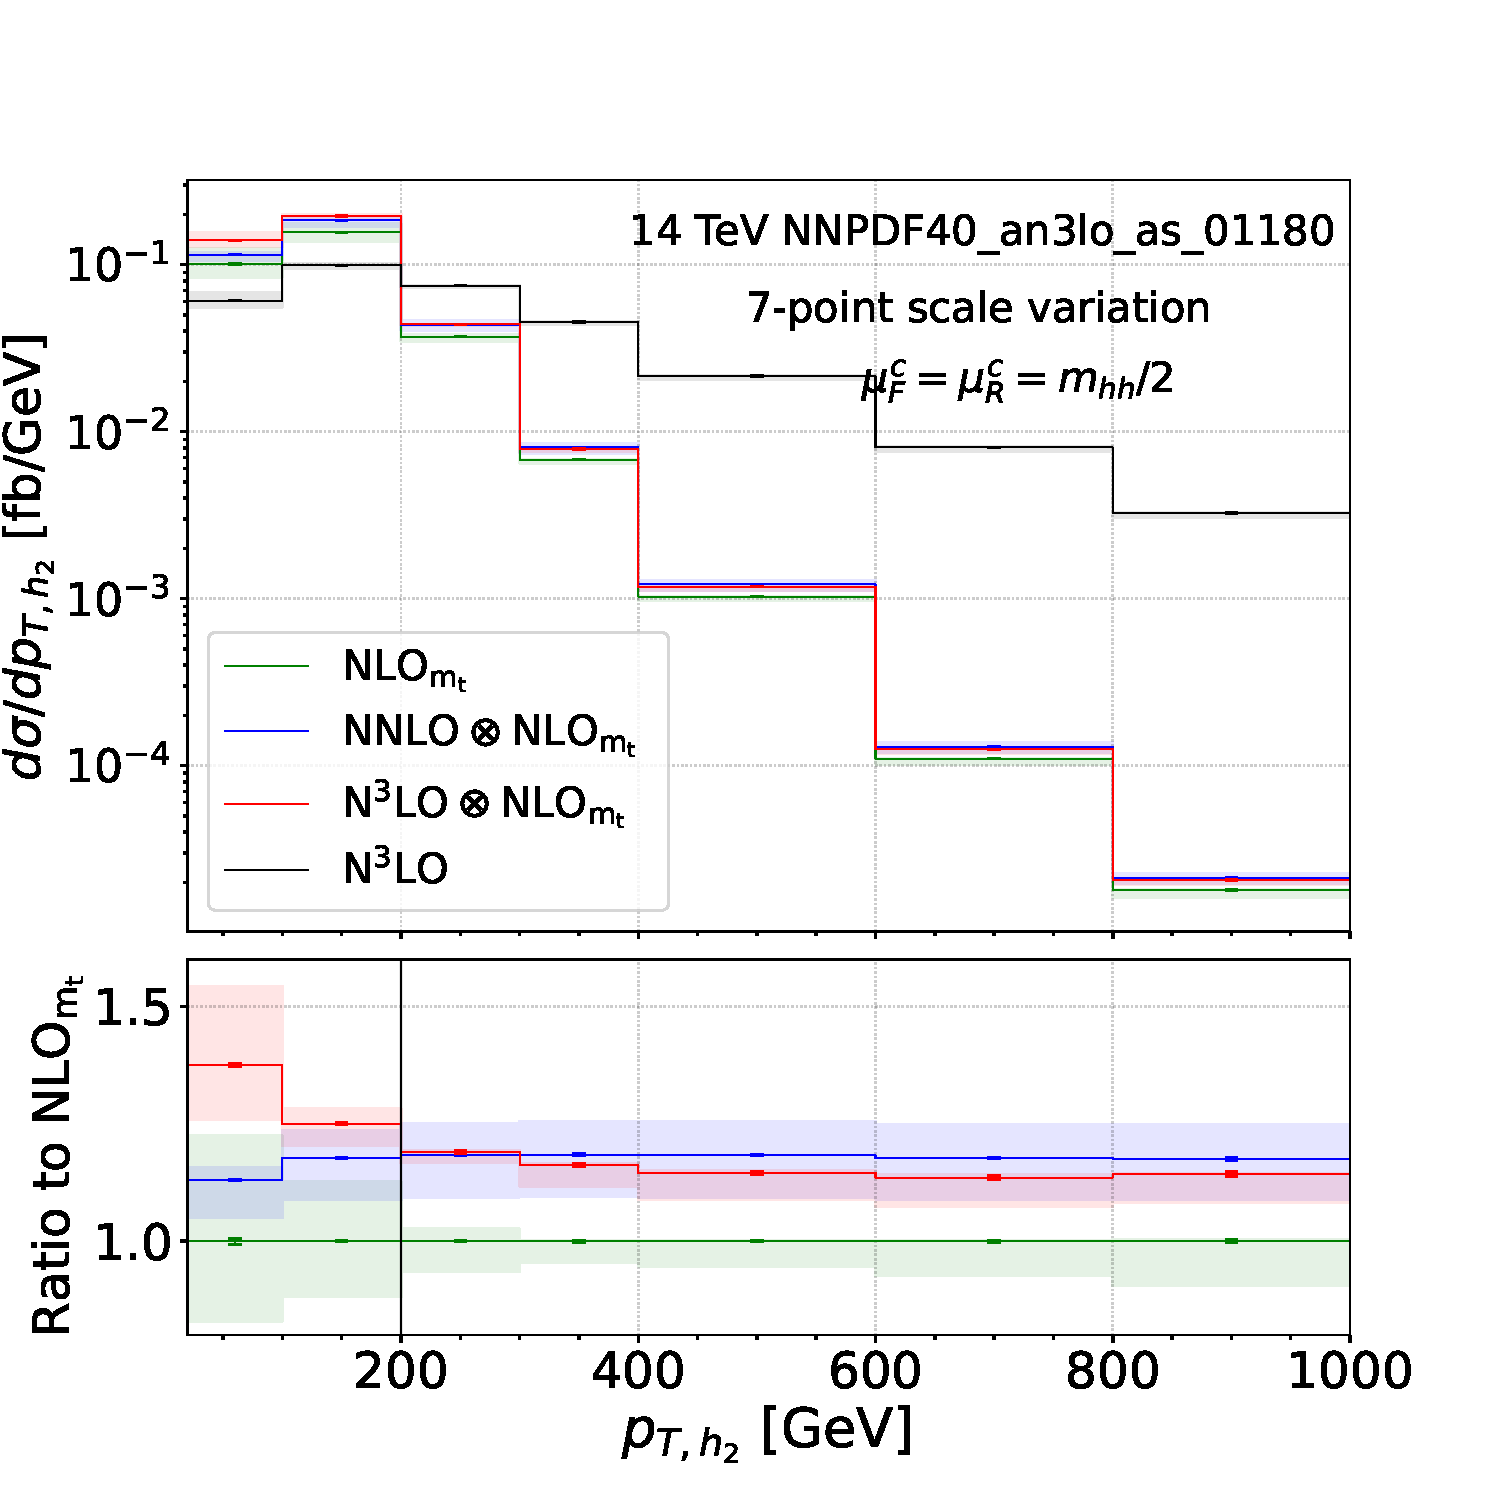
\includegraphics[width=0.49\textwidth,height=7.52cm]{N3LO_QCD_SM/N3LO_mt/Images/HH_pt_h2nd_r.pdf}
\caption{Inclusive (left) and fiducial (right) subleading-Higgs $p_{T}$ distributions for Higgs boson pair production at $\sqrt{s}=14$ TeV, including top quark mass effects. The error bands stem from $7$-point scale variations. Here $\mu^C$ denotes the central value of the renormalization and factorization scales. Results shown are from Ref.~\cite{Chen:2026zmi}.}
\label{fig:fid_pth2_mt}
\end{figure*}

